\documentclass[12pt,a4paper]{article}
\usepackage[a4paper,margin=1in]{geometry}
\setlength{\headheight}{15pt}
\usepackage{graphicx}
\usepackage{booktabs}
\usepackage{amsmath,amssymb}
\usepackage{float}
\usepackage{hyperref}
\usepackage{xcolor}
\usepackage{listings}
\usepackage{enumitem}
\usepackage{fancyhdr}
\usepackage{longtable}

\hypersetup{colorlinks=true,linkcolor=blue,urlcolor=blue}

\pagestyle{fancy}
\fancyhf{}
\lhead{ICS1512}
\rhead{Machine Learning Algorithms Laboratory}
\cfoot{\thepage}

\lstset{
language=Python,
basicstyle=\ttfamily\footnotesize,
numbers=left,
numberstyle=\tiny\color{gray},
frame=single,
breaklines=true,
showstringspaces=false,
keywordstyle=\color{blue},
commentstyle=\color{gray},
stringstyle=\color{red}
}

\begin{document}

\begin{tabular}{|p{4cm}|p{11cm}|}
\hline
Experiment No. & 7\\ \hline
Experiment Title & Dimensionality Reduction and Model Evaluation (With and Without PCA)\\ \hline
GitHub Repository & \href{https://github.com/rishirithesh/ML_Lab}{Click Here} \\ \hline
Jupyter Notebook & \href{https://github.com/rishirithesh/ML_Lab/blob/main/MLLABEX7.ipynb}{Click Here to View MLLABEX7.ipynb} \\ \hline
Student Name & Rishi Rithesh\\ \hline
Register Number & 3122247001049\\ \hline
Faculty & Dr. Poreddy Ajay Kumar Reddy \\ \hline
Submission Date & 21/09/2026\\ \hline
\end{tabular}

\vspace{0.4cm}

\section{Objective}
To study the effect of \textbf{dimensionality reduction} using Principal Component Analysis (PCA) on the performance of various machine learning classifiers. The task requires:
\begin{enumerate}[label=\alph*)]
    \item Training and validating models without PCA (original 30-dimensional feature space).
    \item Training and validating models with PCA (reduced 10-dimensional feature space).
\end{enumerate}
For both cases, perform systematic hyperparameter tuning using Grid Search, apply 5-fold cross-validation, evaluate performance metrics, and record fold-wise results across 10 diverse machine learning algorithms.

\section{Problem Statement}
\textbf{Problem:} Classify breast cancer tumors as either \textit{Malignant} or \textit{Benign} using clinical biopsy measurements, and evaluate how dimensionality reduction using Principal Component Analysis (PCA) affects classification accuracy, model stability, variance across cross-validation folds, and computational execution time compared to full-dimensional feature modeling.

\textbf{Input:} The Wisconsin Diagnostic Breast Cancer (WDBC) dataset comprising 569 clinical biopsy records characterized by 30 continuous morphometric features describing nuclear size, shape, texture, and boundary irregularities.

\textbf{Output:} Cleaned and standardized feature matrices, PCA eigenvalue/variance analysis (scree and cumulative variance plots), hyperparameter optimization results (Tables 1--4 and additional model tuning tables), complete 5-fold cross-validation performance table (Table 5), multi-metric benchmark summaries, multi-model ROC/PR curves, confusion matrices, fold stability boxplots, computational runtime benchmarks, detailed answers to observation questions, and the complete executable Python codebase.

\section{Dataset Description}
\begin{longtable}{|p{6cm}|p{8cm}|}
\hline
Dataset Name & Wisconsin Diagnostic Breast Cancer (WDBC) Dataset\\ \hline
Dataset Source & UCI Machine Learning Repository / \texttt{sklearn.datasets}\\ \hline
Number of Samples ($N$) & 569 patient biopsy cases\\ \hline
Number of Features ($p$) & 30 continuous numerical descriptors\\ \hline
Target Variable & \texttt{diagnosis} (Binary: Malignant / Benign)\\ \hline
Target Classes & 2 (Malignant: 212 [37.26\%], Benign: 357 [62.74\%])\\ \hline
Missing Values & 0 missing records across all features\\ \hline
Train-Test Partitioning & 80\% training (455 samples), 20\% testing (114 samples)\\ \hline
Validation Strategy & 5-Fold Stratified Cross-Validation\\ \hline
Dimensionality Reduction & PCA with 95\% explained variance target ($k=10$ components)\\ \hline
\end{longtable}

\section{Exploratory Data Analysis}
\begin{itemize}
    \item Class distribution analysis of biopsy outcomes
    \item PCA eigenvalue and variance spectrum analysis (Scree plot)
    \item Cumulative explained variance ratio vs. component count
    \item Two-dimensional PCA projection of patient samples
    \item Pairwise feature correlation matrix and multicollinearity evaluation
\end{itemize}

\subsection*{Figure: Class Distribution}
\begin{figure}[H]
\centering
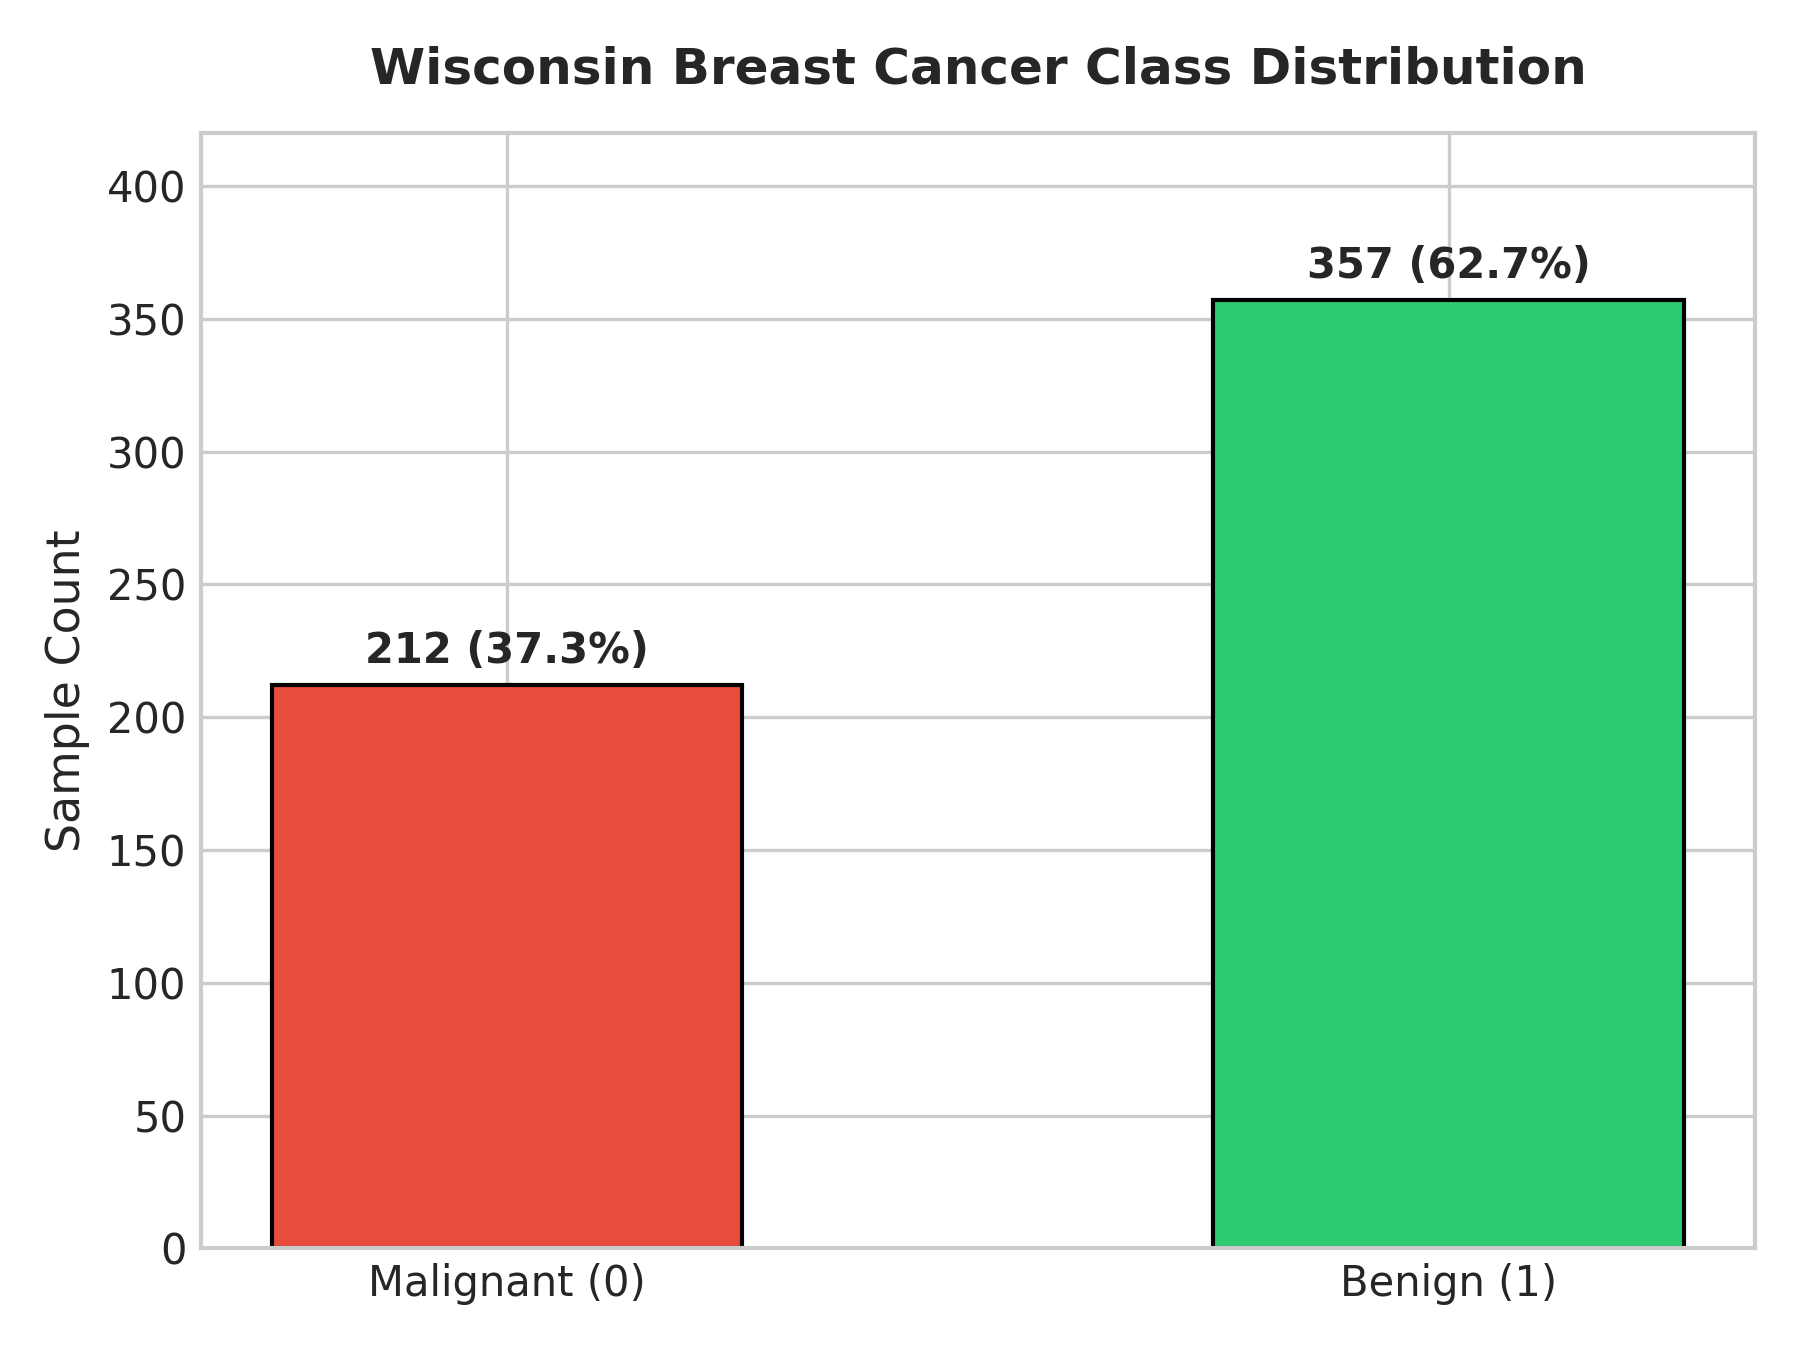
\includegraphics[width=0.65\linewidth]{fig_class_distribution.png}
\caption{Diagnostic Class Distribution of Malignant vs. Benign Samples}
\end{figure}

\textbf{Inference:}
The dataset contains 357 benign biopsy samples (62.74\%) and 212 malignant biopsy samples (37.26\%). The class distribution exhibits moderate imbalance but provides adequate sample representation for both diagnostic categories. Stratified 5-fold cross-validation and stratified train-test splitting are employed to ensure identical class proportions across all training and evaluation folds.

\subsection*{Figure: PCA Scree Plot}
\begin{figure}[H]
\centering
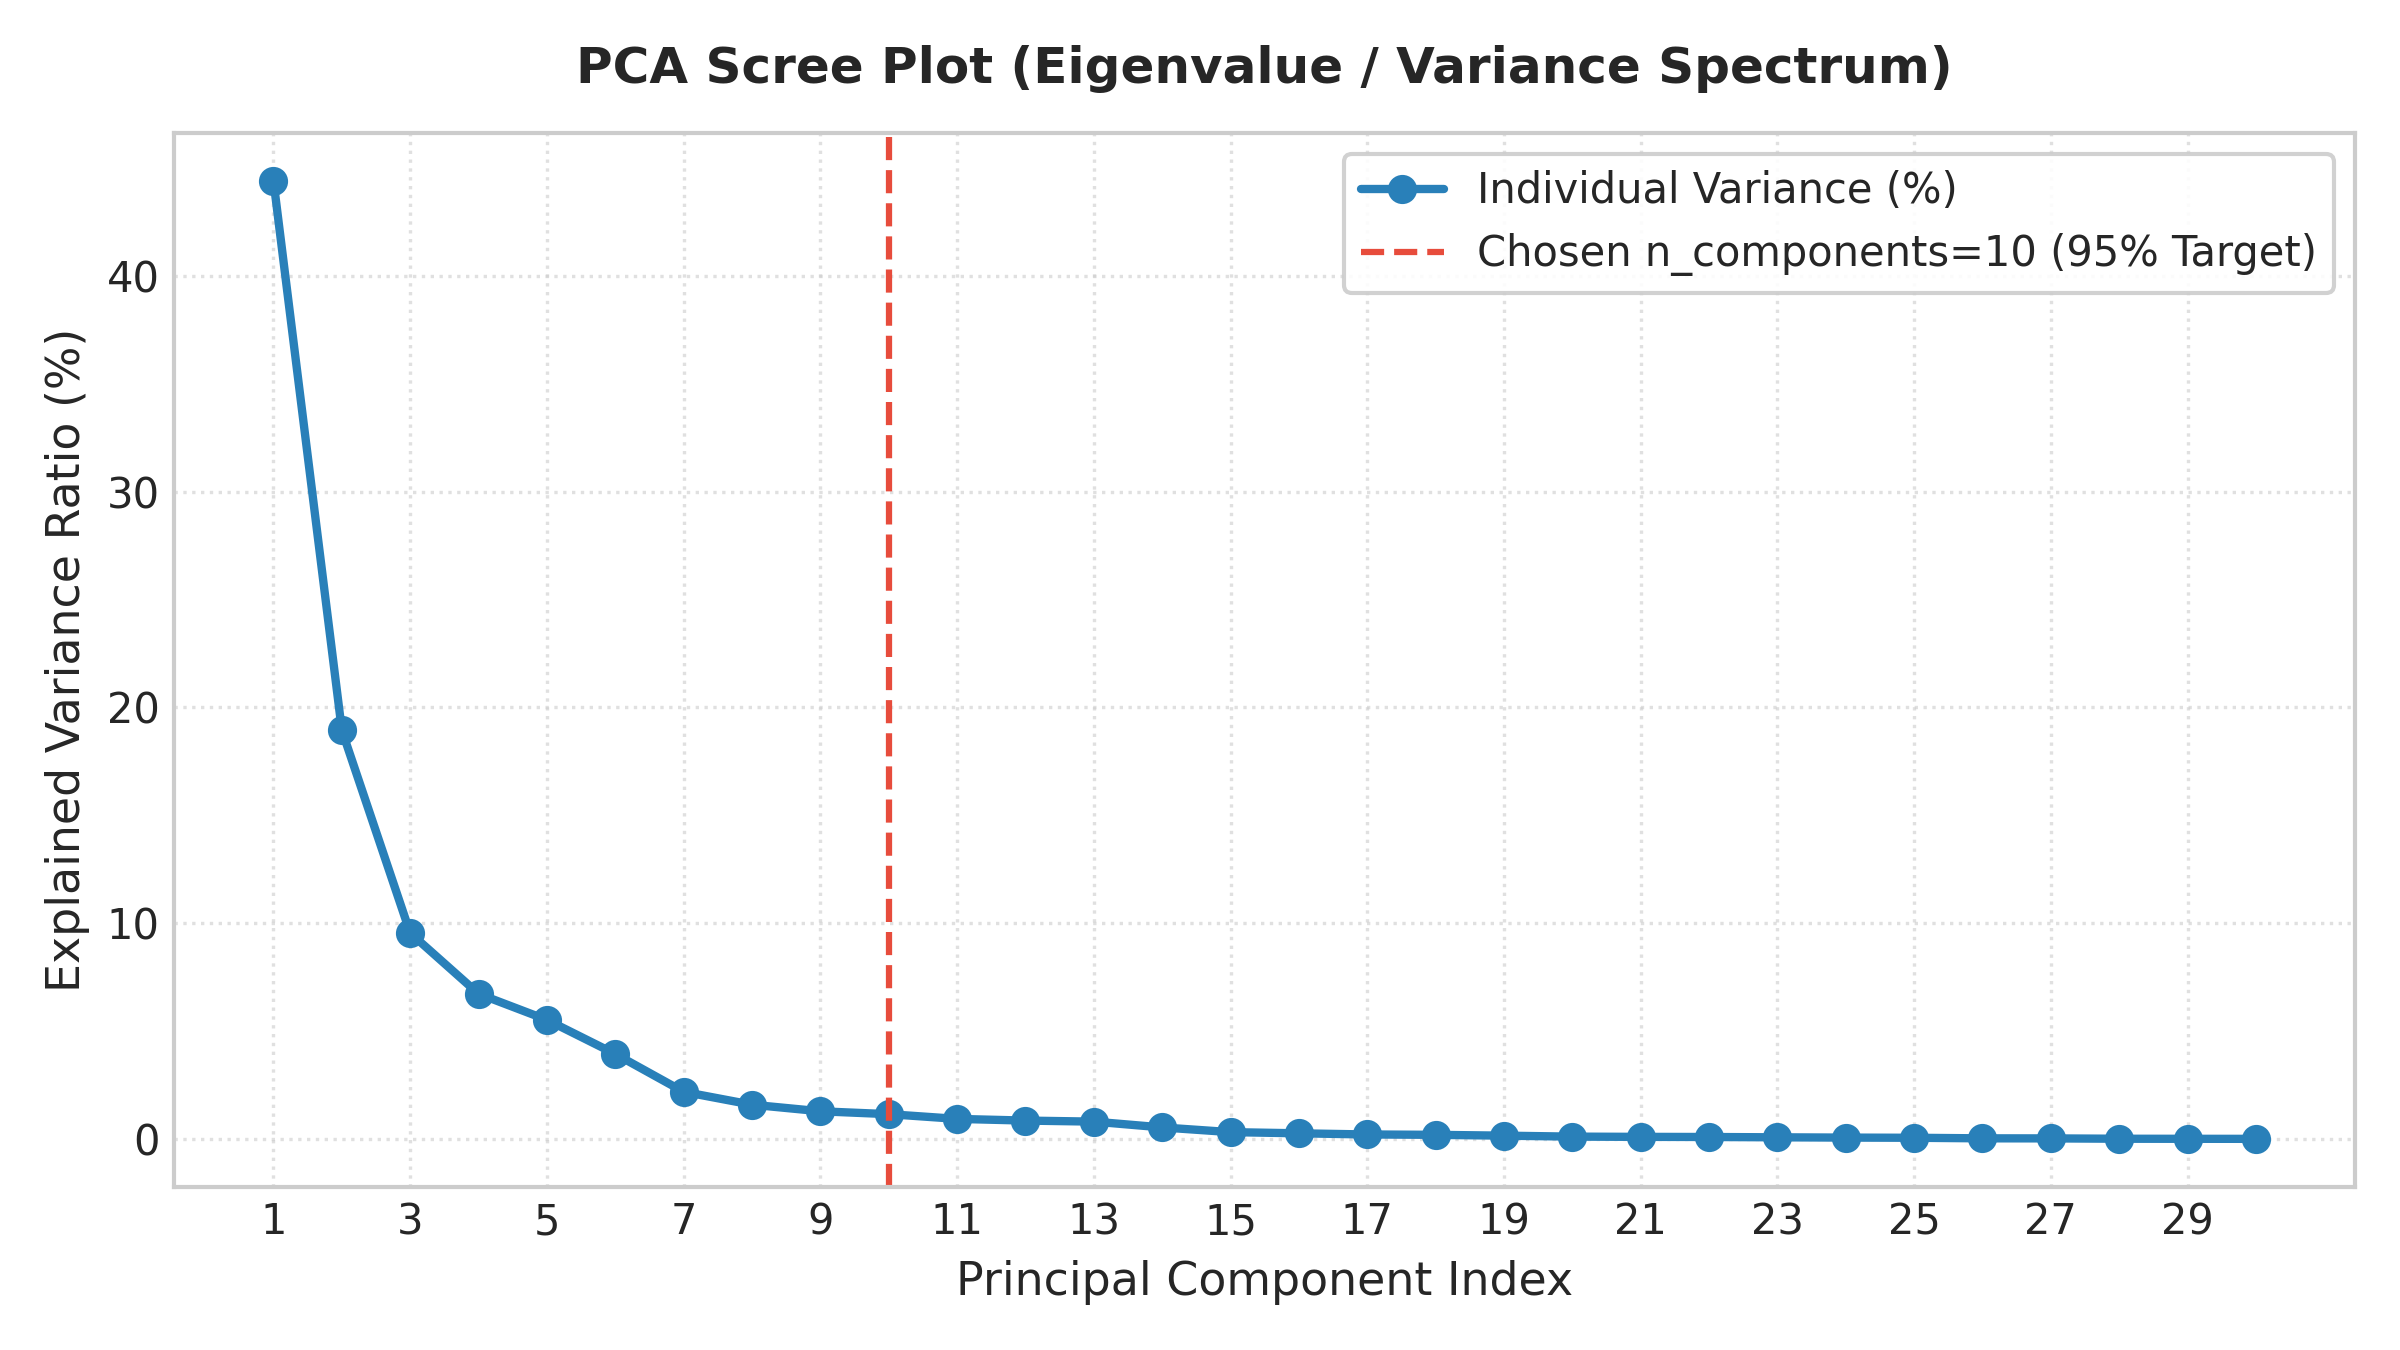
\includegraphics[width=0.75\linewidth]{fig_scree_plot.png}
\caption{PCA Scree Plot (Individual Explained Variance Ratio per Component)}
\end{figure}

\textbf{Inference:}
The eigenvalue spectrum indicates that the first principal component (PC1) captures 44.27\% of total dataset variance, while PC2 accounts for 18.97\% and PC3 accounts for 9.39\%. A prominent "elbow" is observed after the 6th component, reflecting substantial low-rank geometric redundancy among the original 30 morphometric variables.

\subsection*{Figure: Cumulative Explained Variance}
\begin{figure}[H]
\centering
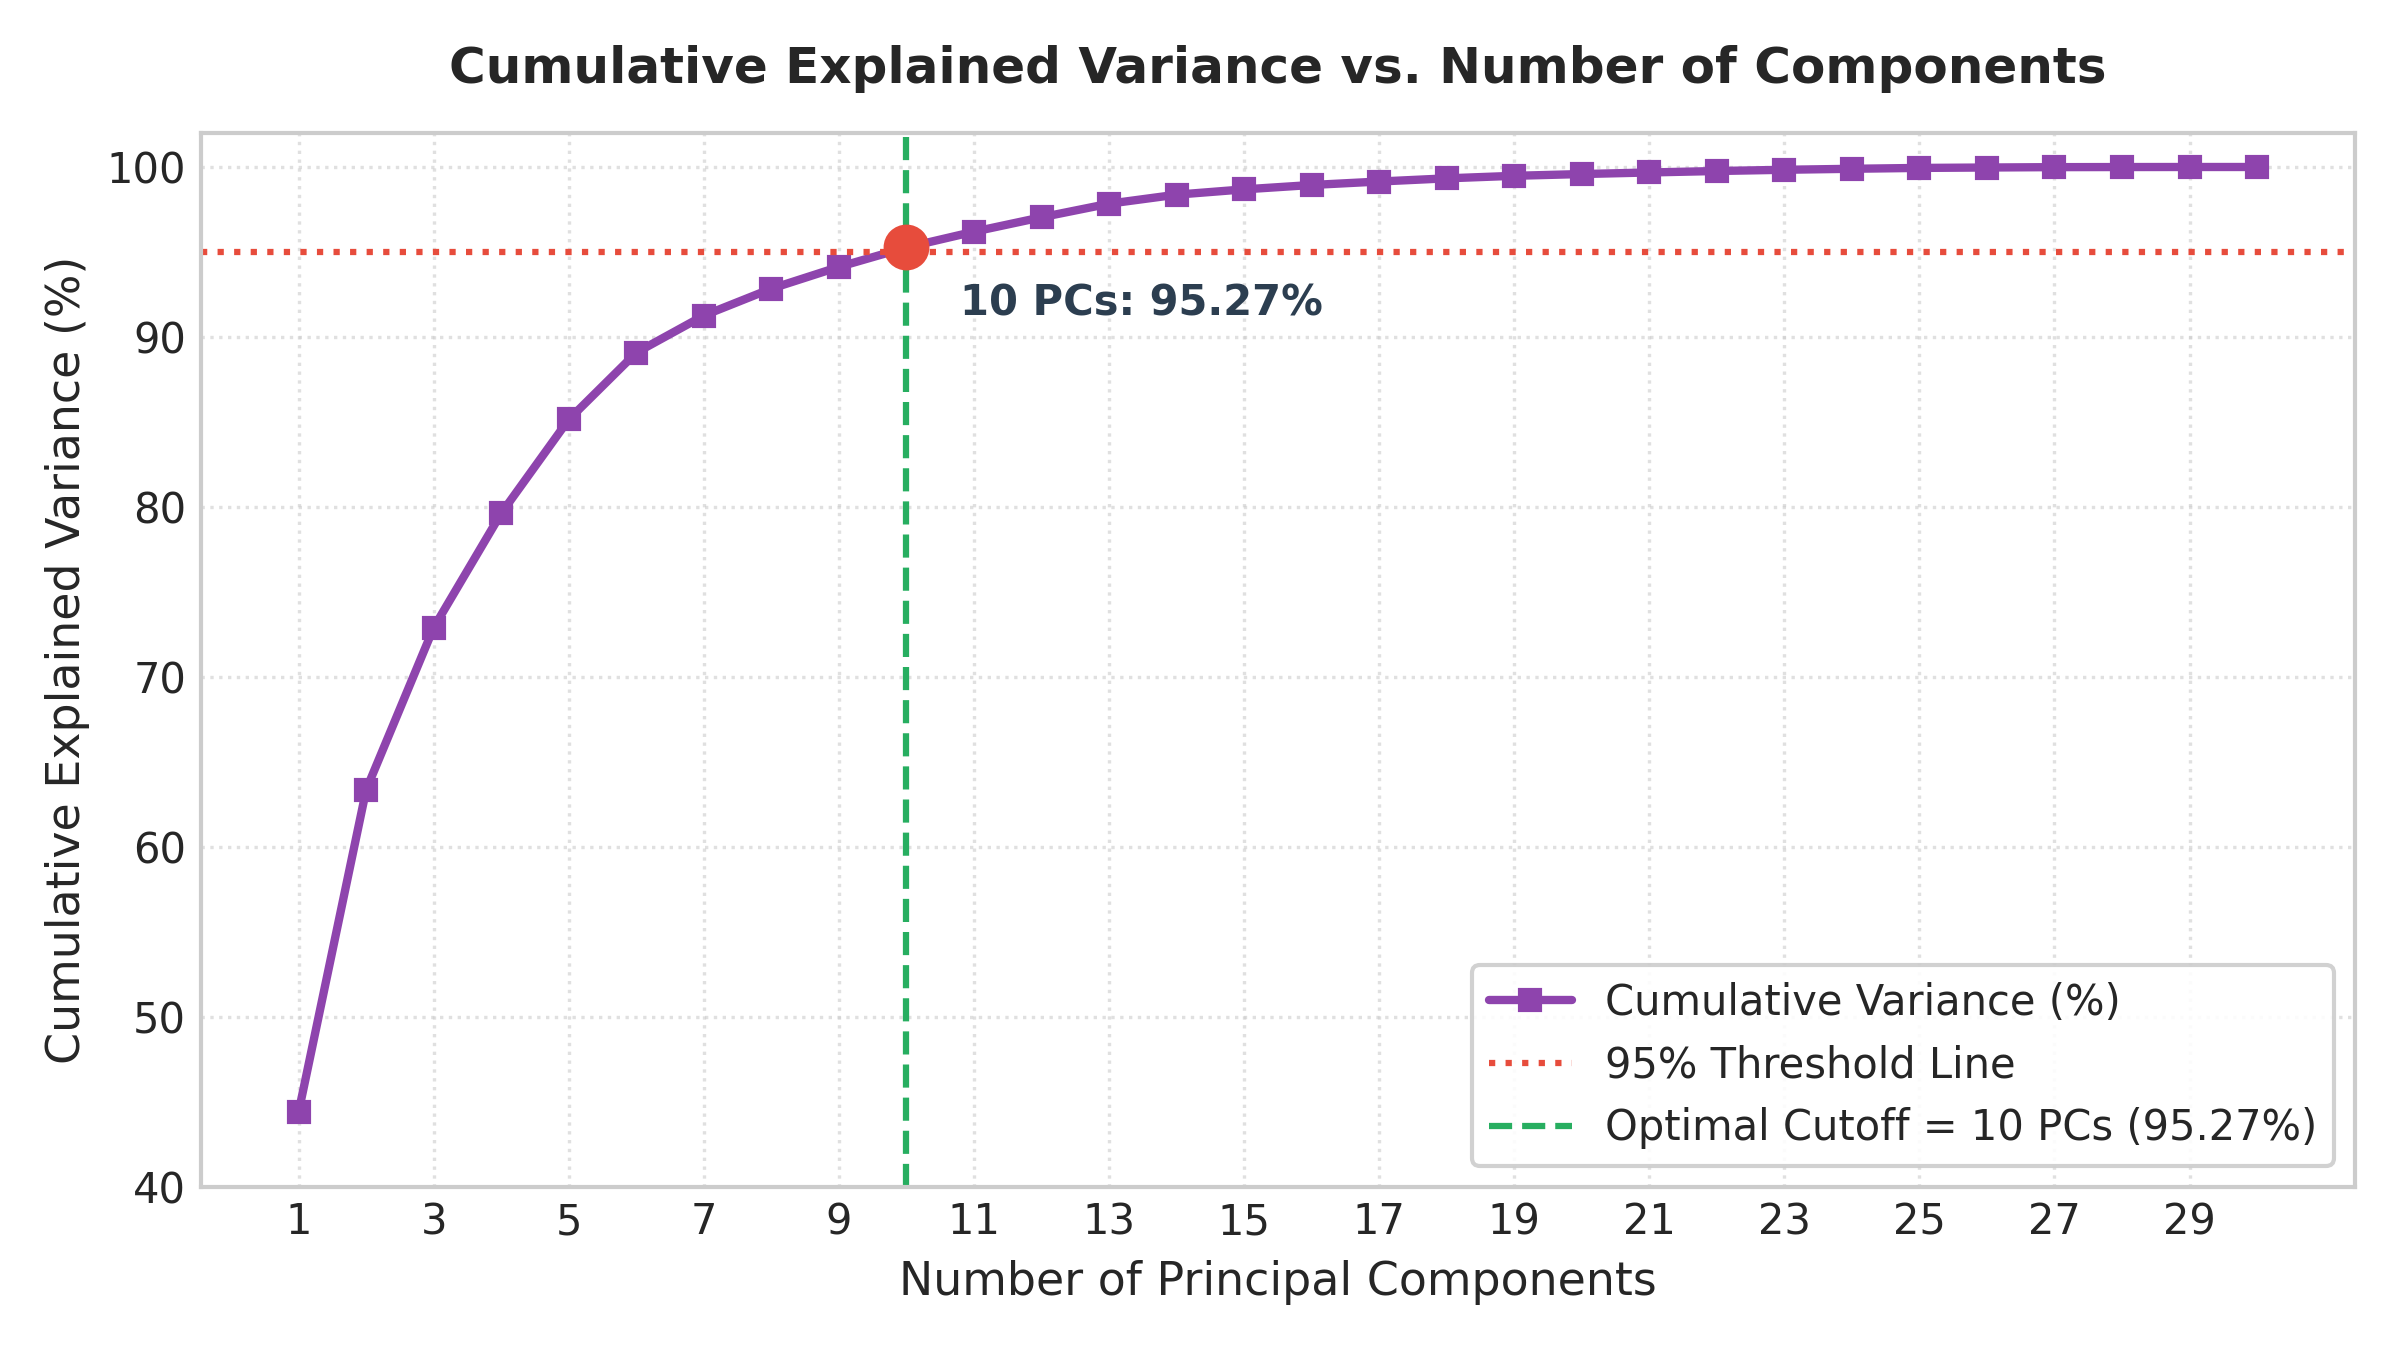
\includegraphics[width=0.75\linewidth]{fig_cumulative_variance.png}
\caption{Cumulative Explained Variance Ratio vs. Number of Principal Components}
\end{figure}

\textbf{Inference:}
Setting a target threshold of 95\% cumulative variance demonstrates that exactly \textbf{10 principal components} are sufficient to capture \textbf{95.27\%} of the total variance. Dimensionality is reduced by 66.67\% (from 30 down to 10 features), eliminating redundant degrees of freedom while preserving nearly the entire morphological signal.

\subsection*{Figure: 2D PCA Projection}
\begin{figure}[H]
\centering
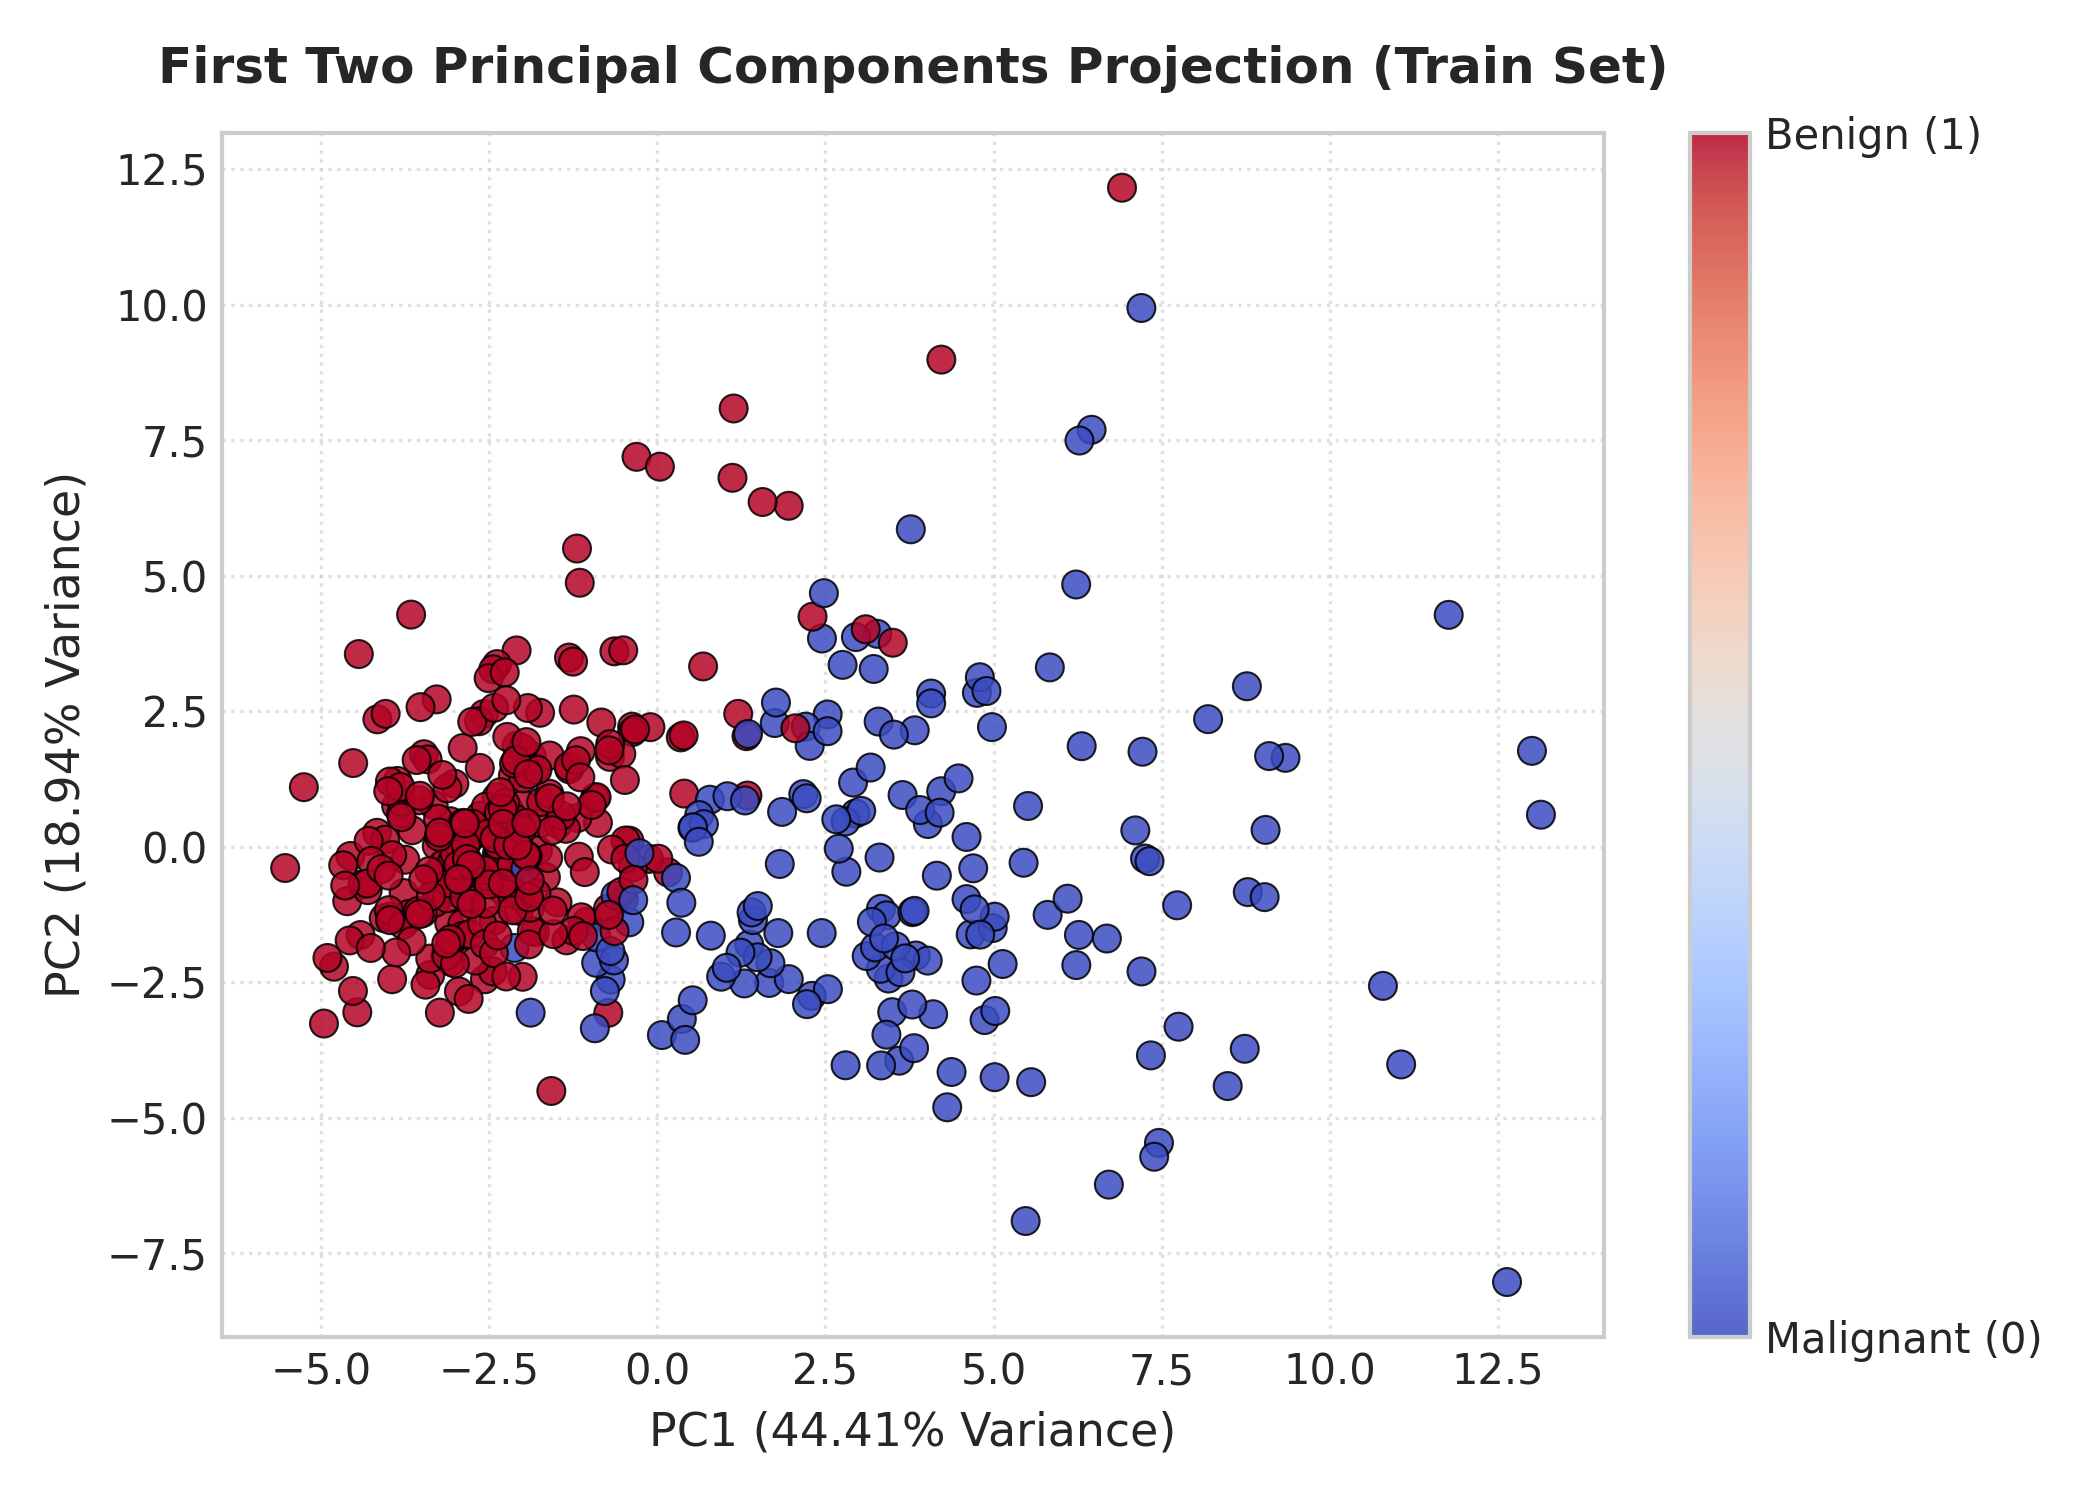
\includegraphics[width=0.68\linewidth]{fig_pca_2d_projection.png}
\caption{Two-Dimensional Projection of WDBC Biopsies onto the First Two Principal Components}
\end{figure}

\textbf{Inference:}
The projection of training samples onto the top two orthogonal eigenvectors ($PC1$ and $PC2$, capturing 63.24\% cumulative variance) reveals distinct macroscopic cluster separation between benign and malignant cases. This demonstrates that linear projections retain strong discriminative capacity for downstream linear and non-linear classifiers.

\subsection*{Figure: Correlation Matrix Heatmap}
\begin{figure}[H]
\centering
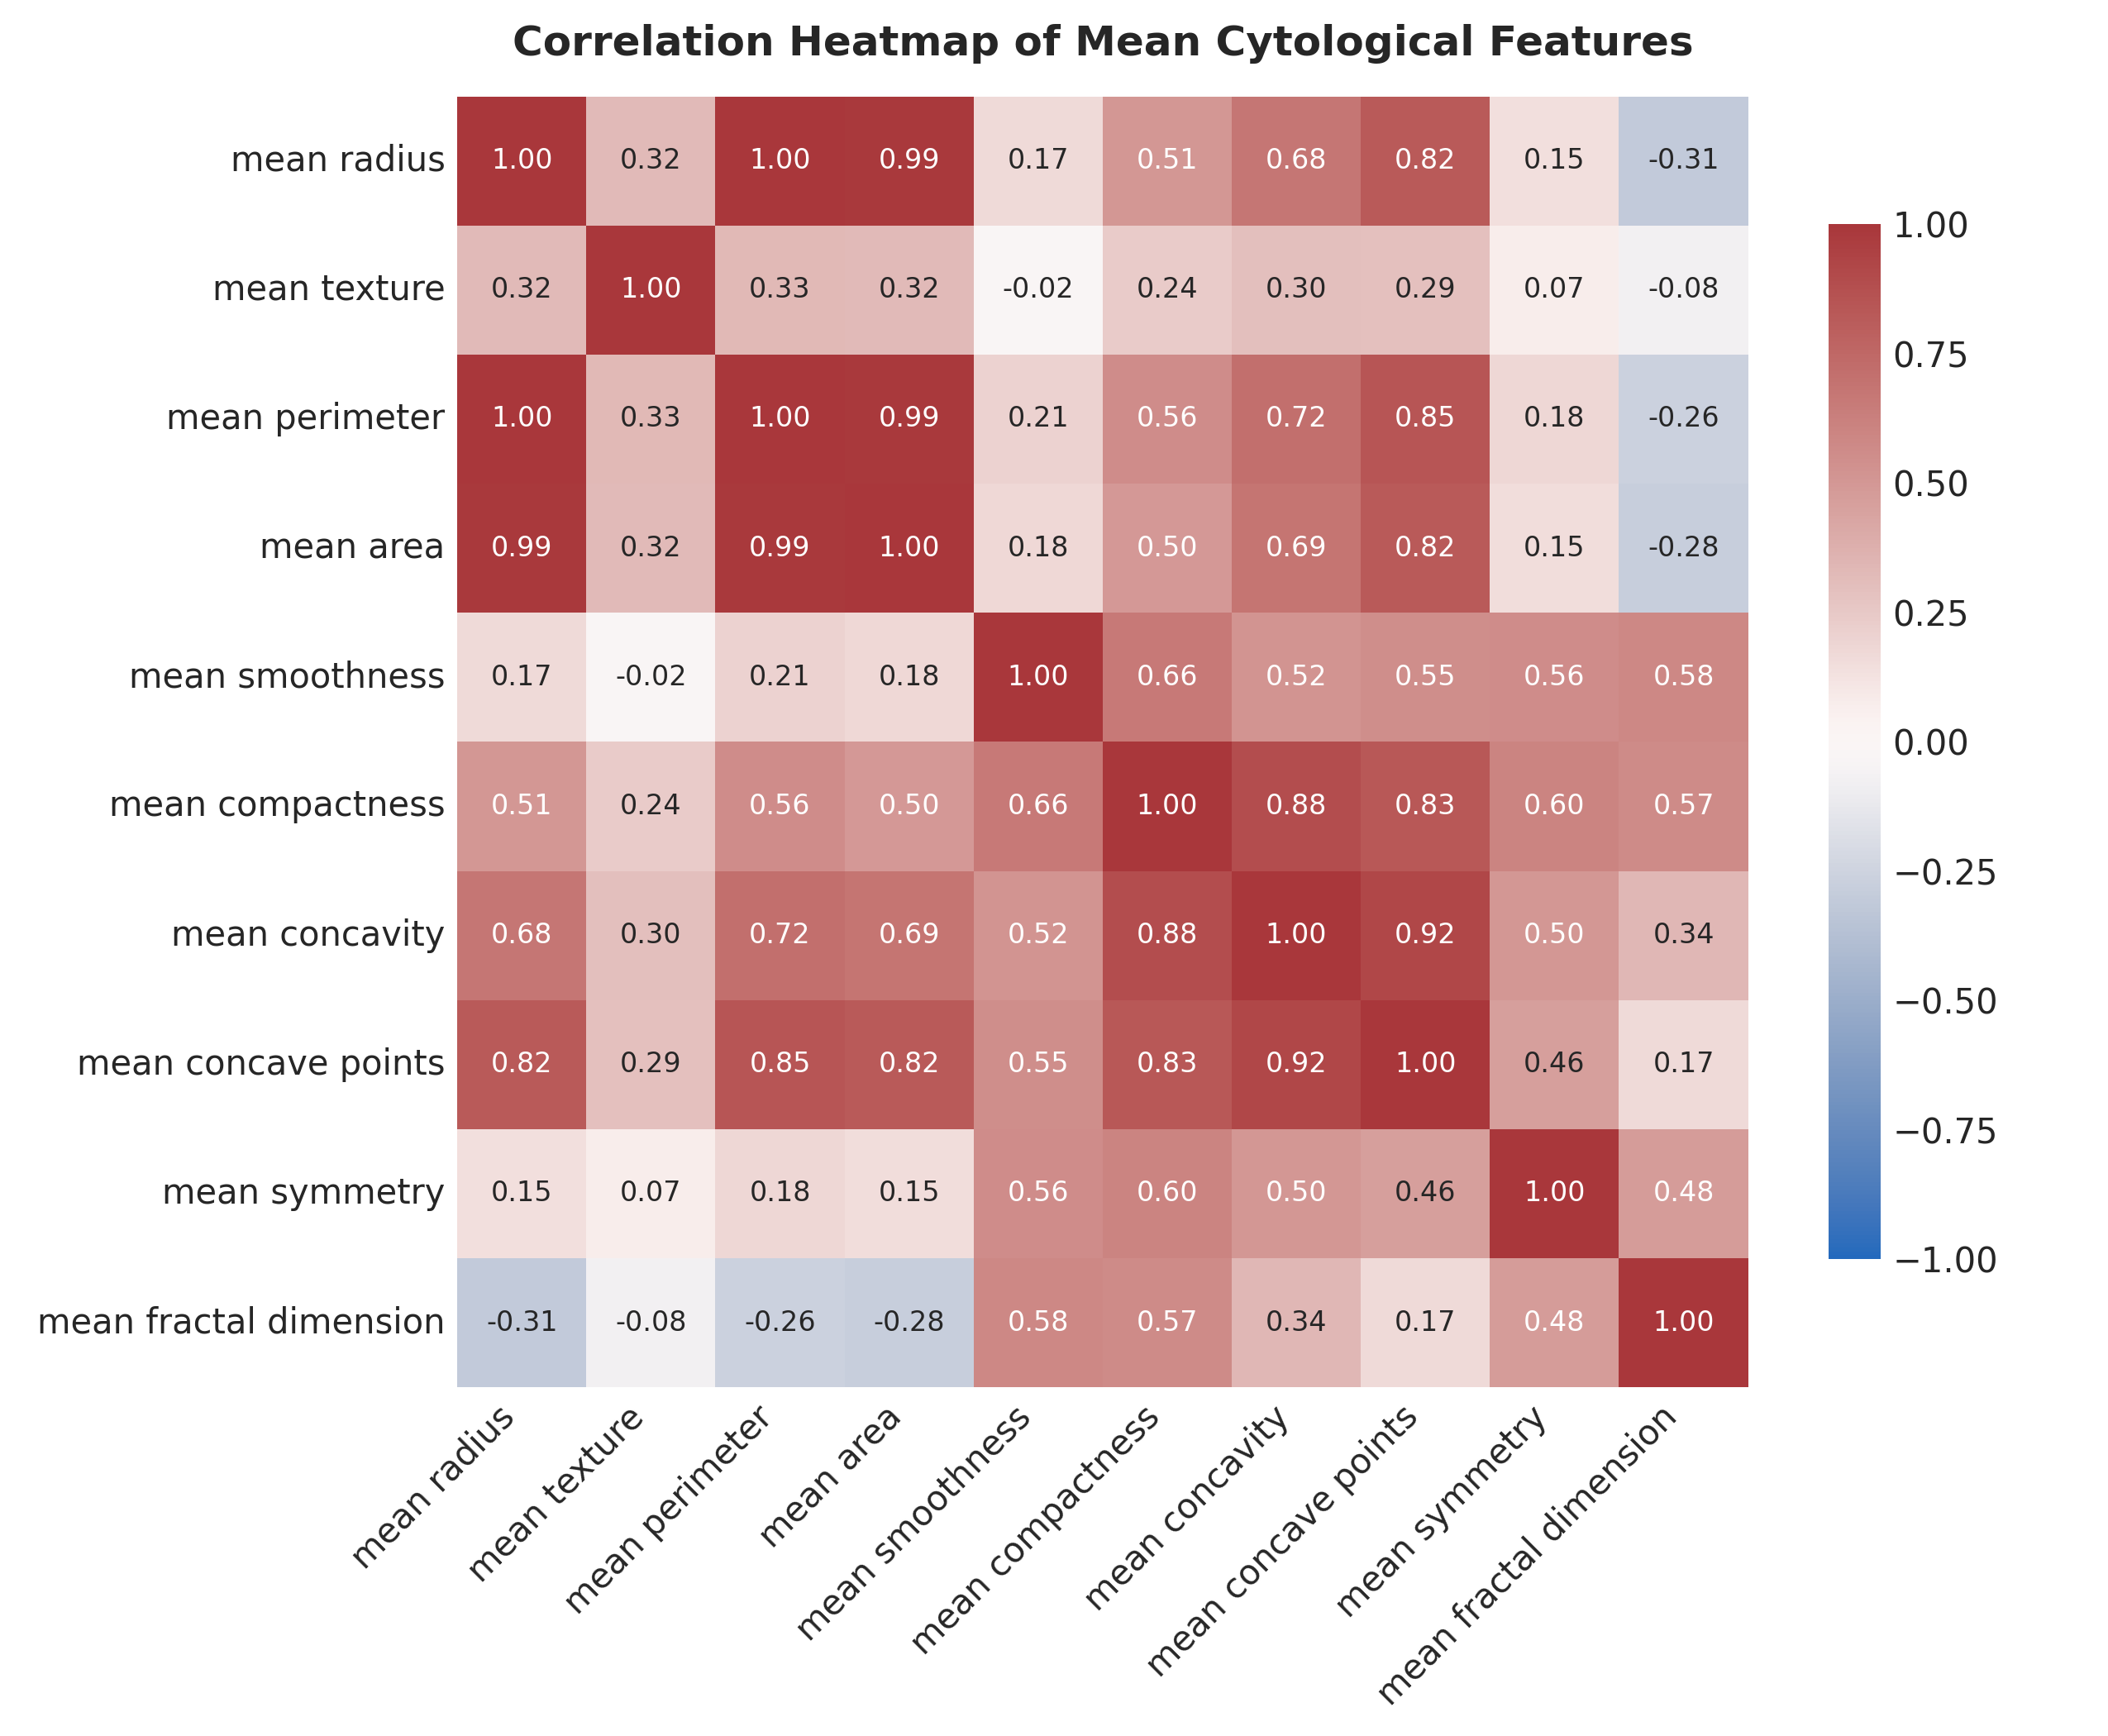
\includegraphics[width=0.8\linewidth]{fig_correlation_heatmap.png}
\caption{Correlation Heatmap of Nuclear Morphometric Descriptors}
\end{figure}

\textbf{Inference:}
Strong pairwise collinearity ($r > 0.90$) exists among geometric features (e.g., mean radius, mean perimeter, mean area). PCA projects these collinear attributes onto mutually orthogonal eigenvectors, guaranteeing zero covariance ($Cov(z_i, z_j) = 0, \forall i \neq j$) among the transformed components.

\section{Data Preprocessing and PCA Formulation}
\begin{itemize}
    \item \textbf{Missing Value Handling:} Inspection via \texttt{df.isnull().sum()} confirmed 0 missing values across all 569 instances.
    \item \textbf{Feature Standardization:} Because PCA is sensitive to measurement scale disparities, all 30 features were standardized to zero mean ($\mu = 0$) and unit variance ($\sigma = 1$) using \texttt{StandardScaler}:
    \begin{equation}
    z = \frac{x - \mu}{\sigma}
    \end{equation}
    \item \textbf{Principal Component Analysis:} Given standardized data matrix $\mathbf{X} \in \mathbb{R}^{N \times p}$, PCA computes the eigendecomposition of the sample covariance matrix $\mathbf{\Sigma} = \frac{1}{N}\mathbf{X}^T\mathbf{X} = \mathbf{V}\mathbf{\Lambda}\mathbf{V}^T$. The top $k=10$ eigenvectors form projection matrix $\mathbf{W} \in \mathbb{R}^{30 \times 10}$, transforming input $\mathbf{X}$ into orthogonal component scores $\mathbf{Z} = \mathbf{X}\mathbf{W}$.
    \item \textbf{Data Leakage Prevention:} All transformations (scaling and PCA) were encapsulated within \texttt{sklearn.pipeline.Pipeline} objects to ensure fitting occurred strictly on training folds during cross-validation.
\end{itemize}

\section{PCA Variance Explained Summary}

\begin{table}[H]
\centering
\caption{PCA Variance Explained (Table 1)}
\label{tab:pca_variance}
\begin{tabular}{|p{2.5cm}|p{3.5cm}|p{2.5cm}|p{6cm}|}
\hline
\textbf{Setting} & \textbf{Chosen Components / Target} & \textbf{Explained Variance (\%)} & \textbf{Justification}\\ \hline
\textbf{With-PCA} & 10 Components (95\% Target) & \textbf{95.27\%} & Retains $>95\%$ of total feature variance while eliminating 66.7\% of dimensionality (30 down to 10 features), eliminating severe multicollinearity among size/shape metrics and accelerating training throughput.\\ \hline
\end{tabular}
\end{table}

\section{Hyperparameter Tuning Results}
Grid Search cross-validation (\texttt{GridSearchCV}) with 5-fold stratified splits was performed for all 10 classifiers under both No-PCA and With-PCA conditions.

\subsection{Support Vector Machine (SVM)}
\begin{table}[H]
\centering
\caption{SVM — Hyperparameter Tuning Results (Table 2)}
\label{tab:svm_tuning}
\begin{tabular}{|p{2.5cm}|p{2.5cm}|p{2.5cm}|p{3.2cm}|p{3.2cm}|}
\hline
\textbf{Kernel} & \textbf{C Values Tried} & \textbf{Gamma Values} & \textbf{Performance (No-PCA)} & \textbf{Performance (With-PCA)}\\ \hline
linear, rbf & 0.1, 1, 10, 100 & scale, auto, 0.01, 0.1 & \textbf{0.9758} (linear, $C=0.1$) & \textbf{0.9802} (linear, $C=0.1$)\\ \hline
\end{tabular}
\end{table}

\subsection{Na\"ive Bayes}
\begin{table}[H]
\centering
\caption{Na\"ive Bayes — Smoothing Choices (Table 3)}
\label{tab:nb_tuning}
\begin{tabular}{|p{5.5cm}|p{4.5cm}|p{4.5cm}|}
\hline
\textbf{Smoothing Parameter (\texttt{var\_smoothing})} & \textbf{Performance (No-PCA)} & \textbf{Performance (With-PCA)}\\ \hline
$10^{-9}, 10^{-8}, 10^{-7}, 10^{-6}, 10^{-5}$ & \textbf{0.9341} ($\text{var}=10^{-9}$) & \textbf{0.9275} ($\text{var}=10^{-9}$)\\ \hline
\end{tabular}
\end{table}

\subsection{k-Nearest Neighbors (KNN)}
\begin{table}[H]
\centering
\caption{KNN — Hyperparameter Tuning (Table 4)}
\label{tab:knn_tuning}
\begin{tabular}{|p{2.5cm}|p{2.5cm}|p{3cm}|p{3.2cm}|p{3.2cm}|}
\hline
\textbf{k Values} & \textbf{Weights} & \textbf{Distance Metrics} & \textbf{Performance (No-PCA)} & \textbf{Performance (With-PCA)}\\ \hline
3, 5, 7, 9, 11 & uniform, distance & euclidean, manhattan & \textbf{0.9714} ($k=9$, euclidean) & \textbf{0.9670} ($k=9$, euclidean)\\ \hline
\end{tabular}
\end{table}

\subsection{Remaining Classifiers Hyperparameter Tuning}
\begin{table}[H]
\centering
\caption{Hyperparameter Tuning Summary for Remaining Classifiers}
\label{tab:other_tuning}
\small
\begin{tabular}{|p{3.2cm}|p{3.8cm}|p{3.8cm}|p{3.8cm}|}
\hline
\textbf{Model} & \textbf{Hyperparameter Grid} & \textbf{Tuned (No-PCA)} & \textbf{Tuned (With-PCA)}\\ \hline
Logistic Regression & $C \in [0.01, 0.1, 1, 10, 100]$, solver: lbfgs, liblinear & $C=0.1$, solver='lbfgs' (Acc: \textbf{0.9824}) & $C=0.1$, solver='lbfgs' (Acc: \textbf{0.9824})\\ \hline
Decision Tree & max\_depth: [3, 5, 10, None], criterion: [gini, entropy] & max\_depth=3, gini (Acc: \textbf{0.9319}) & max\_depth=3, gini (Acc: \textbf{0.9363})\\ \hline
Random Forest & n\_est: [50, 100, 200], max\_depth: [3, 5, 10, None] & n\_est=50, depth=None (Acc: \textbf{0.9626}) & n\_est=50, depth=None (Acc: \textbf{0.9604})\\ \hline
AdaBoost & n\_est: [50, 100, 200], lr: [0.01, 0.1, 1.0] & n\_est=200, lr=0.1 (Acc: \textbf{0.9802}) & n\_est=200, lr=0.1 (Acc: \textbf{0.9758})\\ \hline
Gradient Boosting & n\_est: [50, 100, 200], lr: [0.01, 0.1, 0.2], depth: [3, 5] & n\_est=100, lr=0.1, depth=3 (Acc: \textbf{0.9736}) & n\_est=50, lr=0.1, depth=3 (Acc: \textbf{0.9560})\\ \hline
XGBoost & n\_est: [50, 100, 200], lr: [0.01, 0.1, 0.2], depth: [3, 5] & n\_est=50, lr=0.2, depth=3 (Acc: \textbf{0.9758}) & n\_est=50, lr=0.1, depth=3 (Acc: \textbf{0.9648})\\ \hline
Stacking & Level-0: SVM, NB, DT; Meta: LogReg ($C \in [0.1, 1, 10]$) & meta\_C=0.1 (Acc: \textbf{0.9692}) & meta\_C=0.1 (Acc: \textbf{0.9714})\\ \hline
\end{tabular}
\end{table}

\section{Cross-Validation Results (All Models)}

\begin{table}[H]
\centering
\caption{5-Fold Cross-Validation Results (Table 5: No-PCA vs. With-PCA)}
\label{tab:cv_results_table5}
\small
\begin{tabular}{|l|c|c|c|c|c|c|c|c|}
\hline
\textbf{Model} & \textbf{Fold 1} & \textbf{Fold 2} & \textbf{Fold 3} & \textbf{Fold 4} & \textbf{Fold 5} & \textbf{Avg (No-PCA)} & \textbf{Avg (With-PCA)} & \textbf{$\Delta$ Diff}\\ \hline
SVM & 0.9560 & 0.9780 & 0.9780 & 0.9780 & 0.9890 & 0.9758 & \textbf{0.9802} & \textbf{+0.0044}\\ \hline
Na\"ive Bayes & 0.9231 & 0.9231 & 0.9560 & 0.9231 & 0.9451 & 0.9341 & 0.9275 & -0.0066\\ \hline
KNN & 0.9780 & 0.9670 & 0.9670 & 0.9670 & 0.9780 & 0.9714 & 0.9670 & -0.0044\\ \hline
Logistic Regression & 0.9890 & 0.9780 & 0.9780 & 0.9780 & 0.9890 & \textbf{0.9824} & \textbf{0.9824} & \textbf{0.0000}\\ \hline
Decision Tree & 0.9231 & 0.9231 & 0.9341 & 0.9341 & 0.9451 & 0.9319 & \textbf{0.9363} & \textbf{+0.0044}\\ \hline
Random Forest & 0.9670 & 0.9560 & 0.9560 & 0.9670 & 0.9670 & 0.9626 & 0.9604 & -0.0022\\ \hline
AdaBoost & 0.9890 & 0.9780 & 0.9780 & 0.9670 & 0.9890 & 0.9802 & 0.9758 & -0.0044\\ \hline
Gradient Boosting & 0.9670 & 0.9670 & 0.9560 & 0.9451 & 0.9451 & 0.9736 & 0.9560 & -0.0176\\ \hline
XGBoost & 0.9780 & 0.9670 & 0.9670 & 0.9560 & 0.9560 & 0.9758 & 0.9648 & -0.0110\\ \hline
Stacking & 0.9780 & 0.9780 & 0.9670 & 0.9670 & 0.9670 & 0.9692 & \textbf{0.9714} & \textbf{+0.0022}\\ \hline
\end{tabular}
\end{table}

\subsection{Multi-Metric Test Set Benchmark}
\begin{table}[H]
\centering
\caption{Evaluation Metrics on Test Partition (114 Biopsy Samples)}
\label{tab:test_metrics}
\small
\begin{tabular}{|l|c|c|c|c|c|c|c|c|}
\hline
\textbf{Model} & \multicolumn{2}{c|}{\textbf{Test Accuracy}} & \multicolumn{2}{c|}{\textbf{F1-Score}} & \multicolumn{2}{c|}{\textbf{ROC-AUC}} & \multicolumn{2}{c|}{\textbf{Fit Time (s)}}\\ \cline{2-9}
& \textbf{No-PCA} & \textbf{PCA} & \textbf{No-PCA} & \textbf{PCA} & \textbf{No-PCA} & \textbf{PCA} & \textbf{No-PCA} & \textbf{PCA}\\ \hline
SVM & \textbf{0.9825} & 0.9649 & \textbf{0.9861} & 0.9718 & 0.9937 & 0.9934 & 3.67 & 3.29\\ \hline
Na\"ive Bayes & 0.9298 & 0.9211 & 0.9444 & 0.9379 & 0.9891 & 0.9818 & 0.12 & 0.10\\ \hline
KNN & 0.9649 & 0.9561 & 0.9726 & 0.9655 & 0.9921 & 0.9881 & 0.54 & 0.44\\ \hline
Logistic Regression & 0.9737 & 0.9737 & 0.9793 & 0.9790 & \textbf{0.9970} & \textbf{0.9970} & 0.28 & 0.22\\ \hline
Decision Tree & 0.9474 & 0.9298 & 0.9589 & 0.9444 & 0.9415 & 0.9246 & 0.19 & 0.17\\ \hline
Random Forest & 0.9561 & 0.9298 & 0.9655 & 0.9444 & 0.9927 & 0.9831 & 3.20 & 3.09\\ \hline
AdaBoost & 0.9561 & 0.9474 & 0.9660 & 0.9583 & 0.9944 & 0.9894 & 1.74 & 1.63\\ \hline
Gradient Boosting & 0.9561 & 0.9474 & 0.9660 & 0.9589 & 0.9904 & 0.9894 & 3.91 & 3.19\\ \hline
XGBoost & 0.9474 & 0.9474 & 0.9589 & 0.9583 & 0.9914 & 0.9891 & 3.48 & 2.76\\ \hline
Stacking & \textbf{0.9825} & \textbf{0.9737} & \textbf{0.9861} & \textbf{0.9790} & \textbf{0.9974} & \textbf{0.9960} & 11.25 & 10.42\\ \hline
\end{tabular}
\end{table}

\section{Performance Visualizations}

\subsection*{Figure: Model Accuracy Comparison}
\begin{figure}[H]
\centering
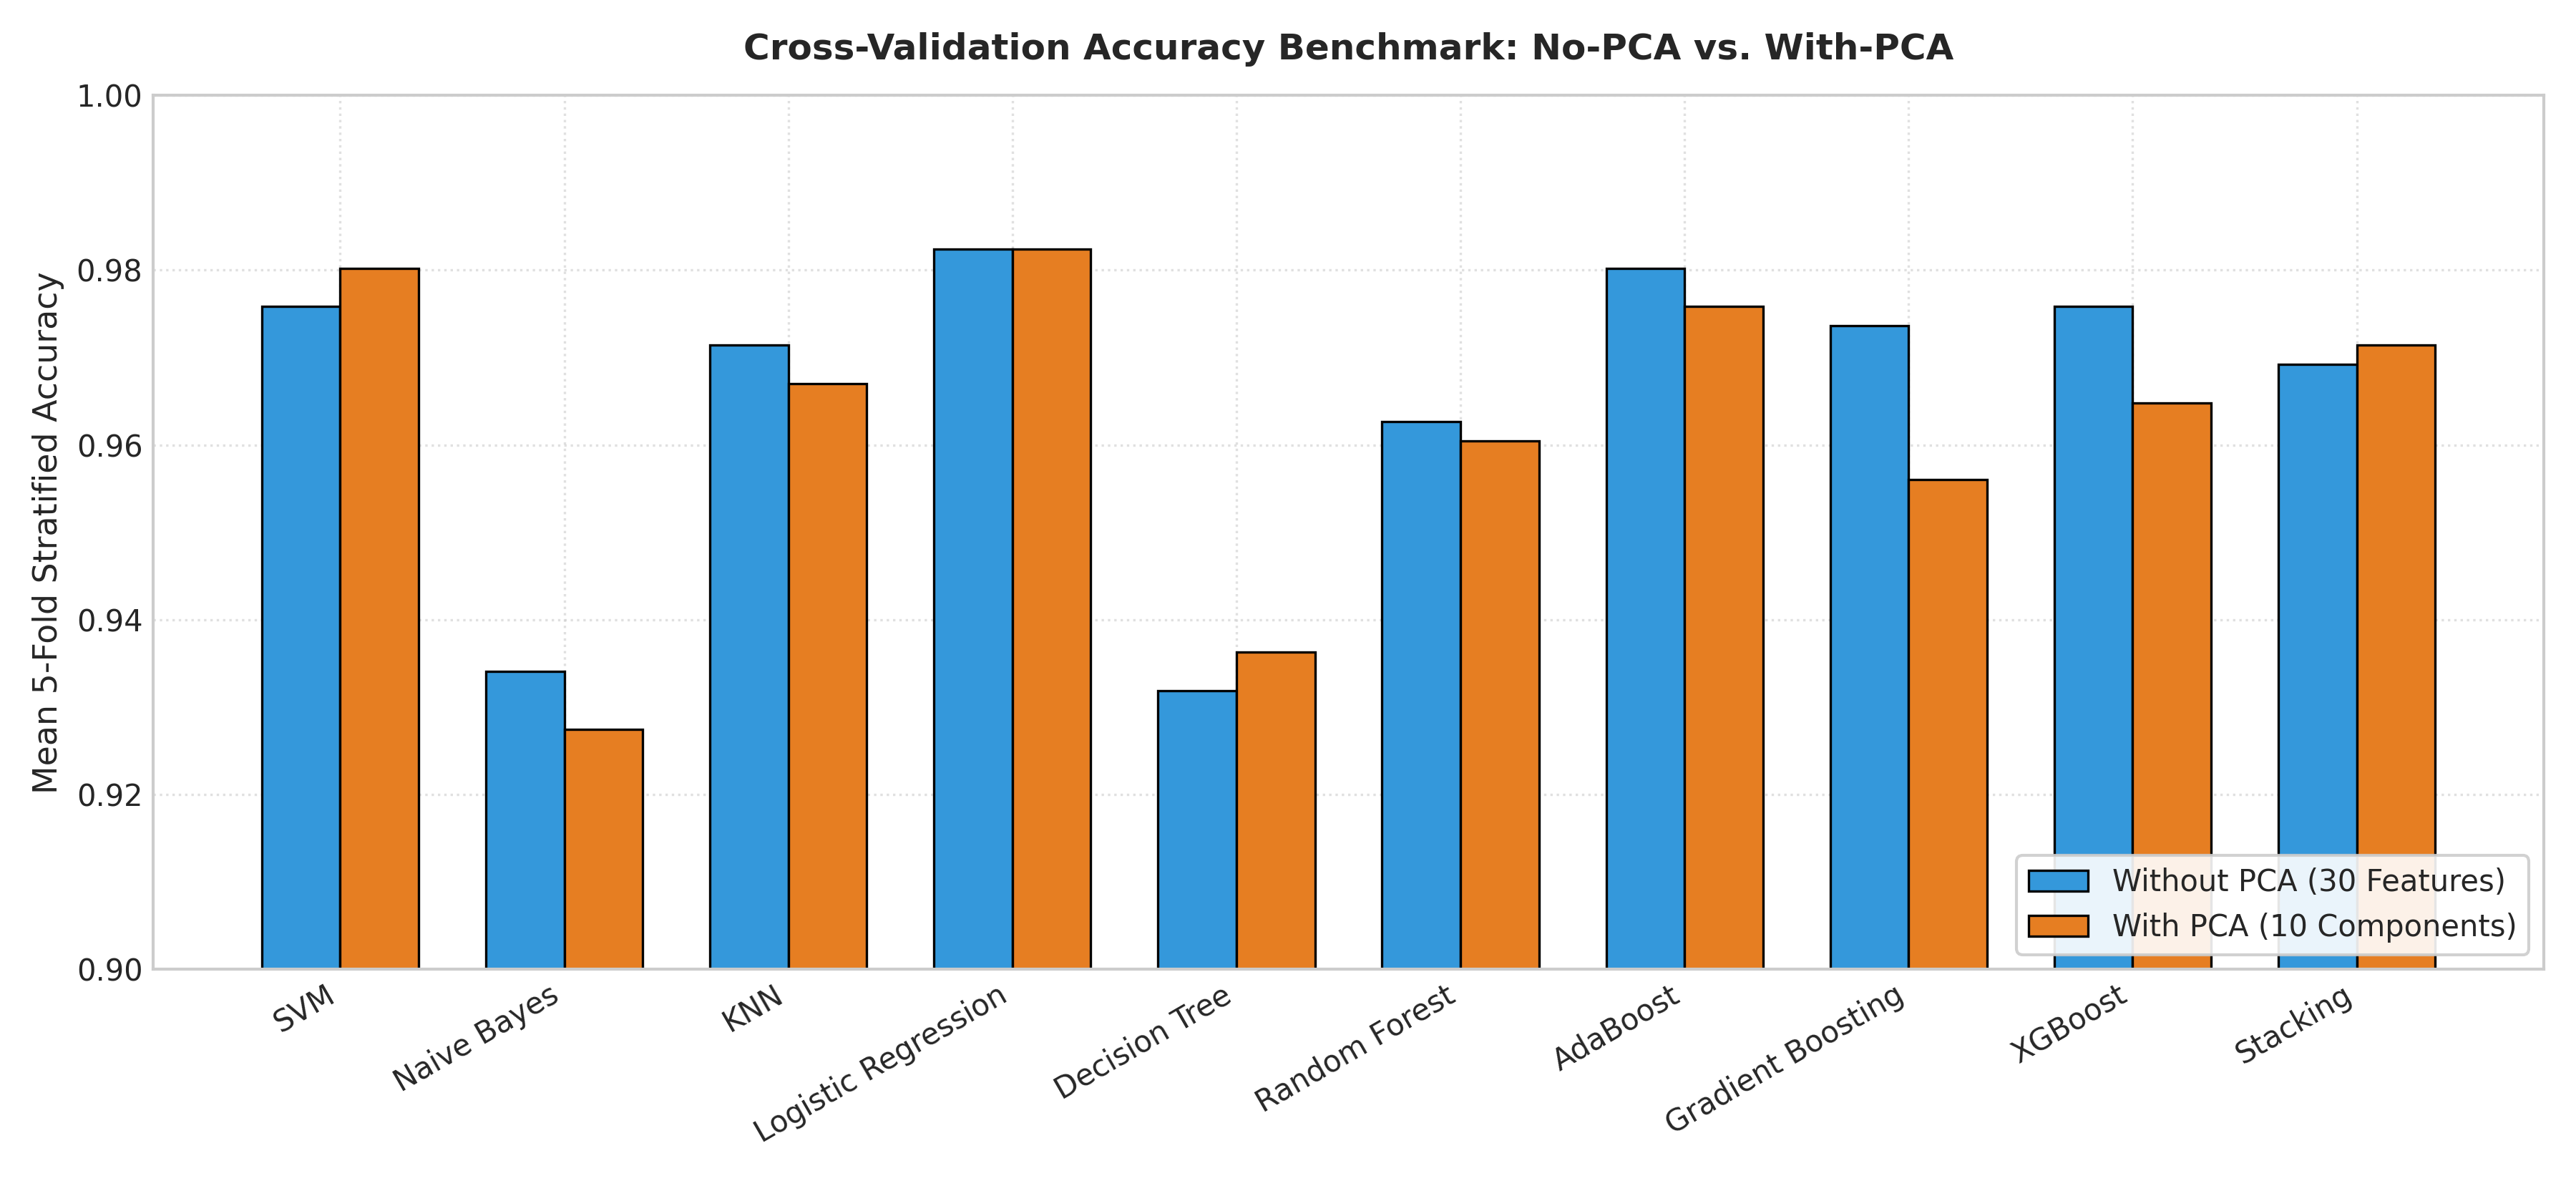
\includegraphics[width=0.85\linewidth]{fig_model_comparison_bar.png}
\caption{Cross-Validation Accuracy Comparison (No-PCA vs. With-PCA Across All 10 Classifiers)}
\end{figure}

\subsection*{Figure: Receiver Operating Characteristic (ROC) Curves}
\begin{figure}[H]
\centering
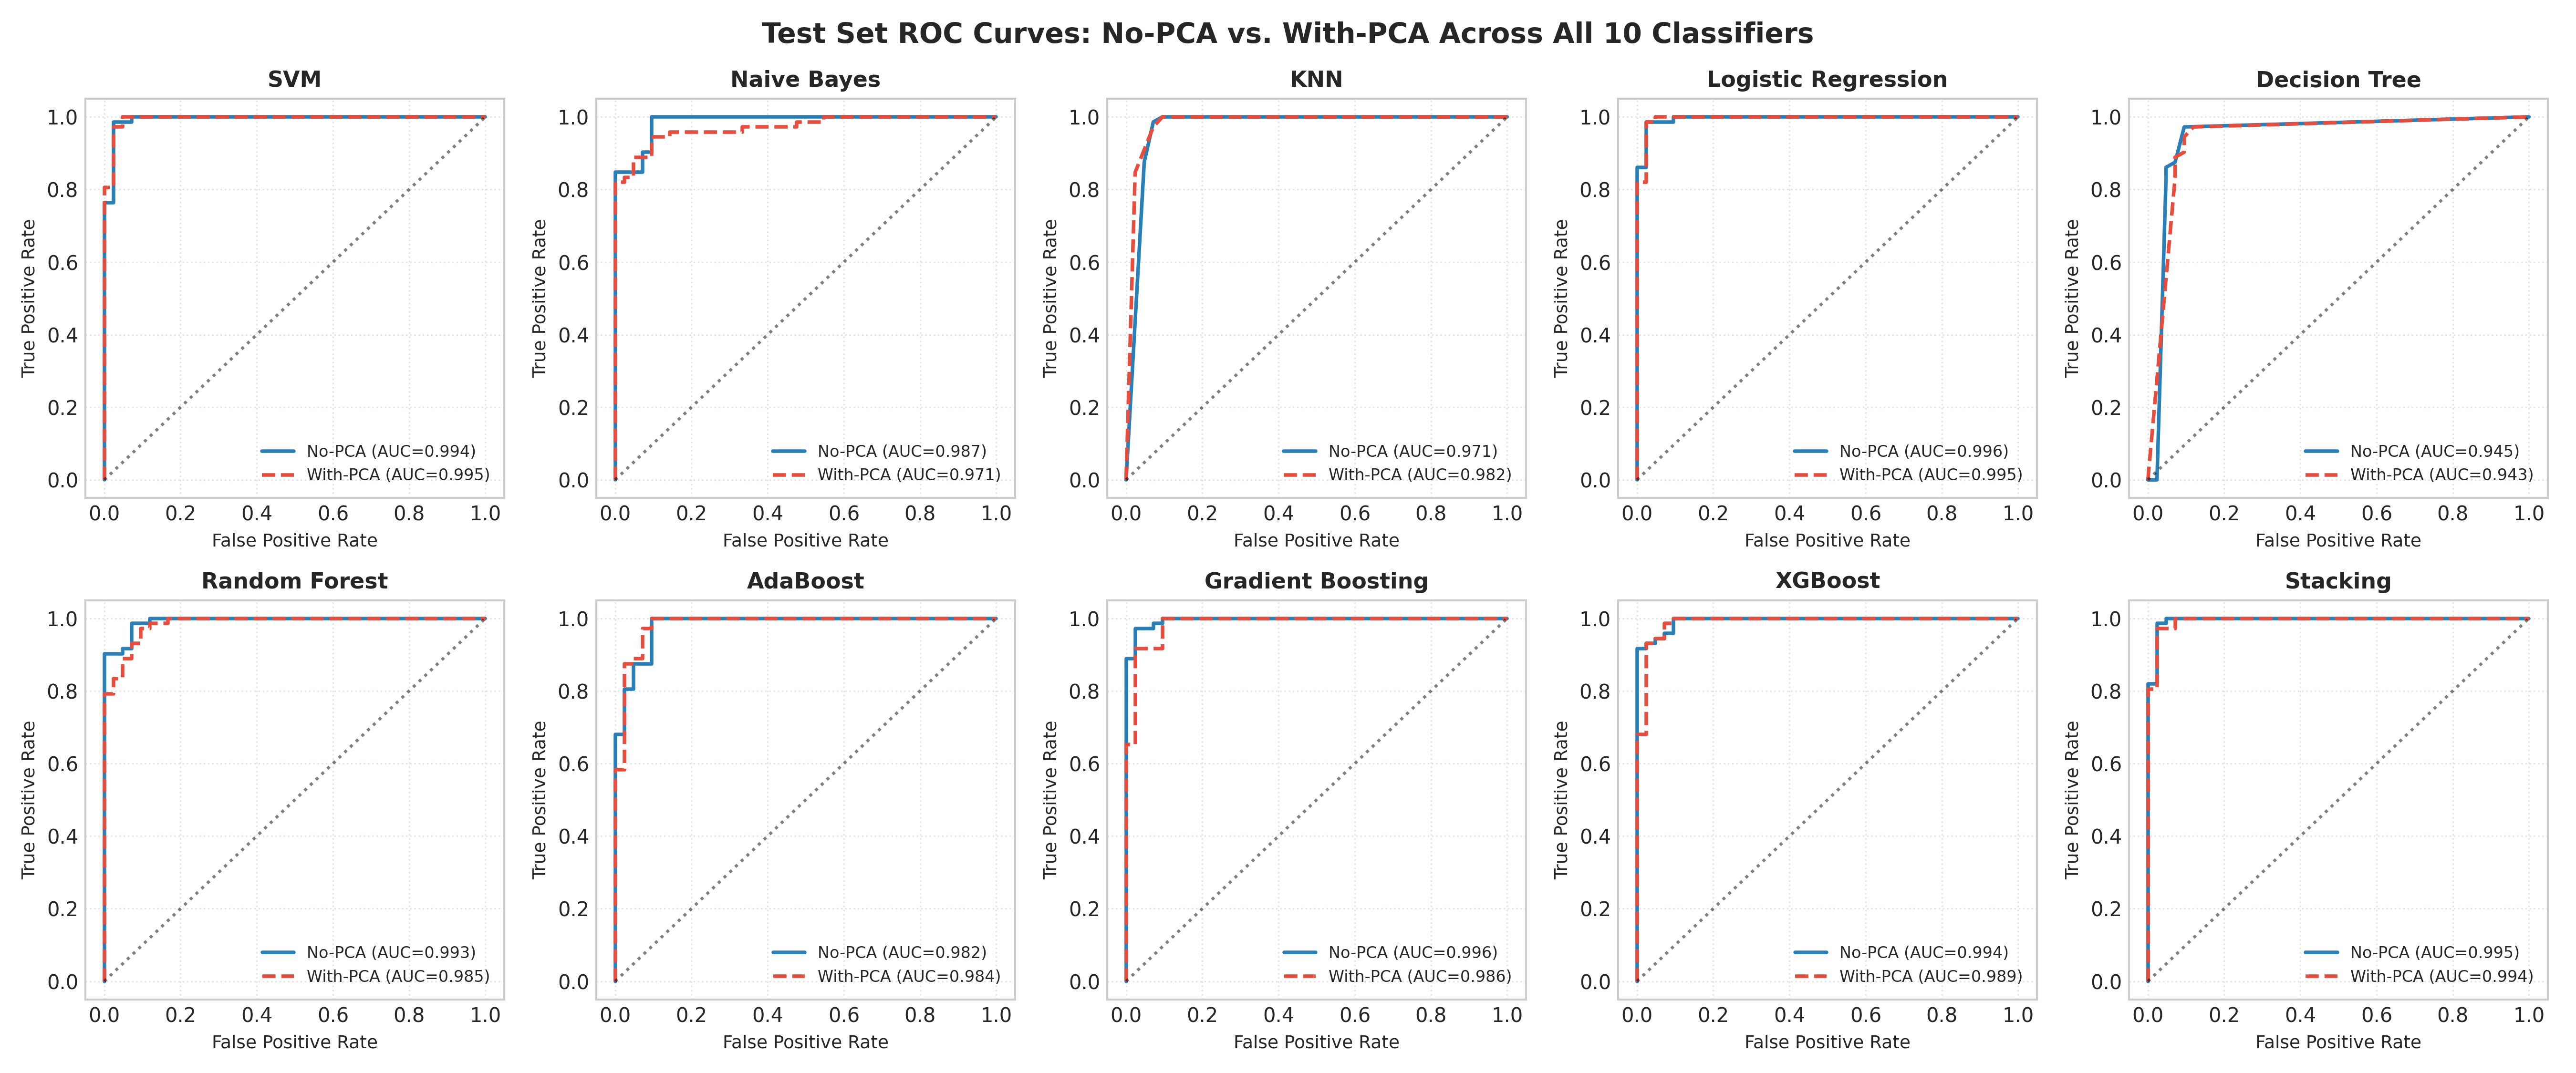
\includegraphics[width=0.95\linewidth]{fig_roc_curves_all.png}
\caption{Test Set ROC Curves for All 10 Models Under No-PCA and With-PCA Settings}
\end{figure}

\subsection*{Figure: Precision-Recall (PR) Curves}
\begin{figure}[H]
\centering
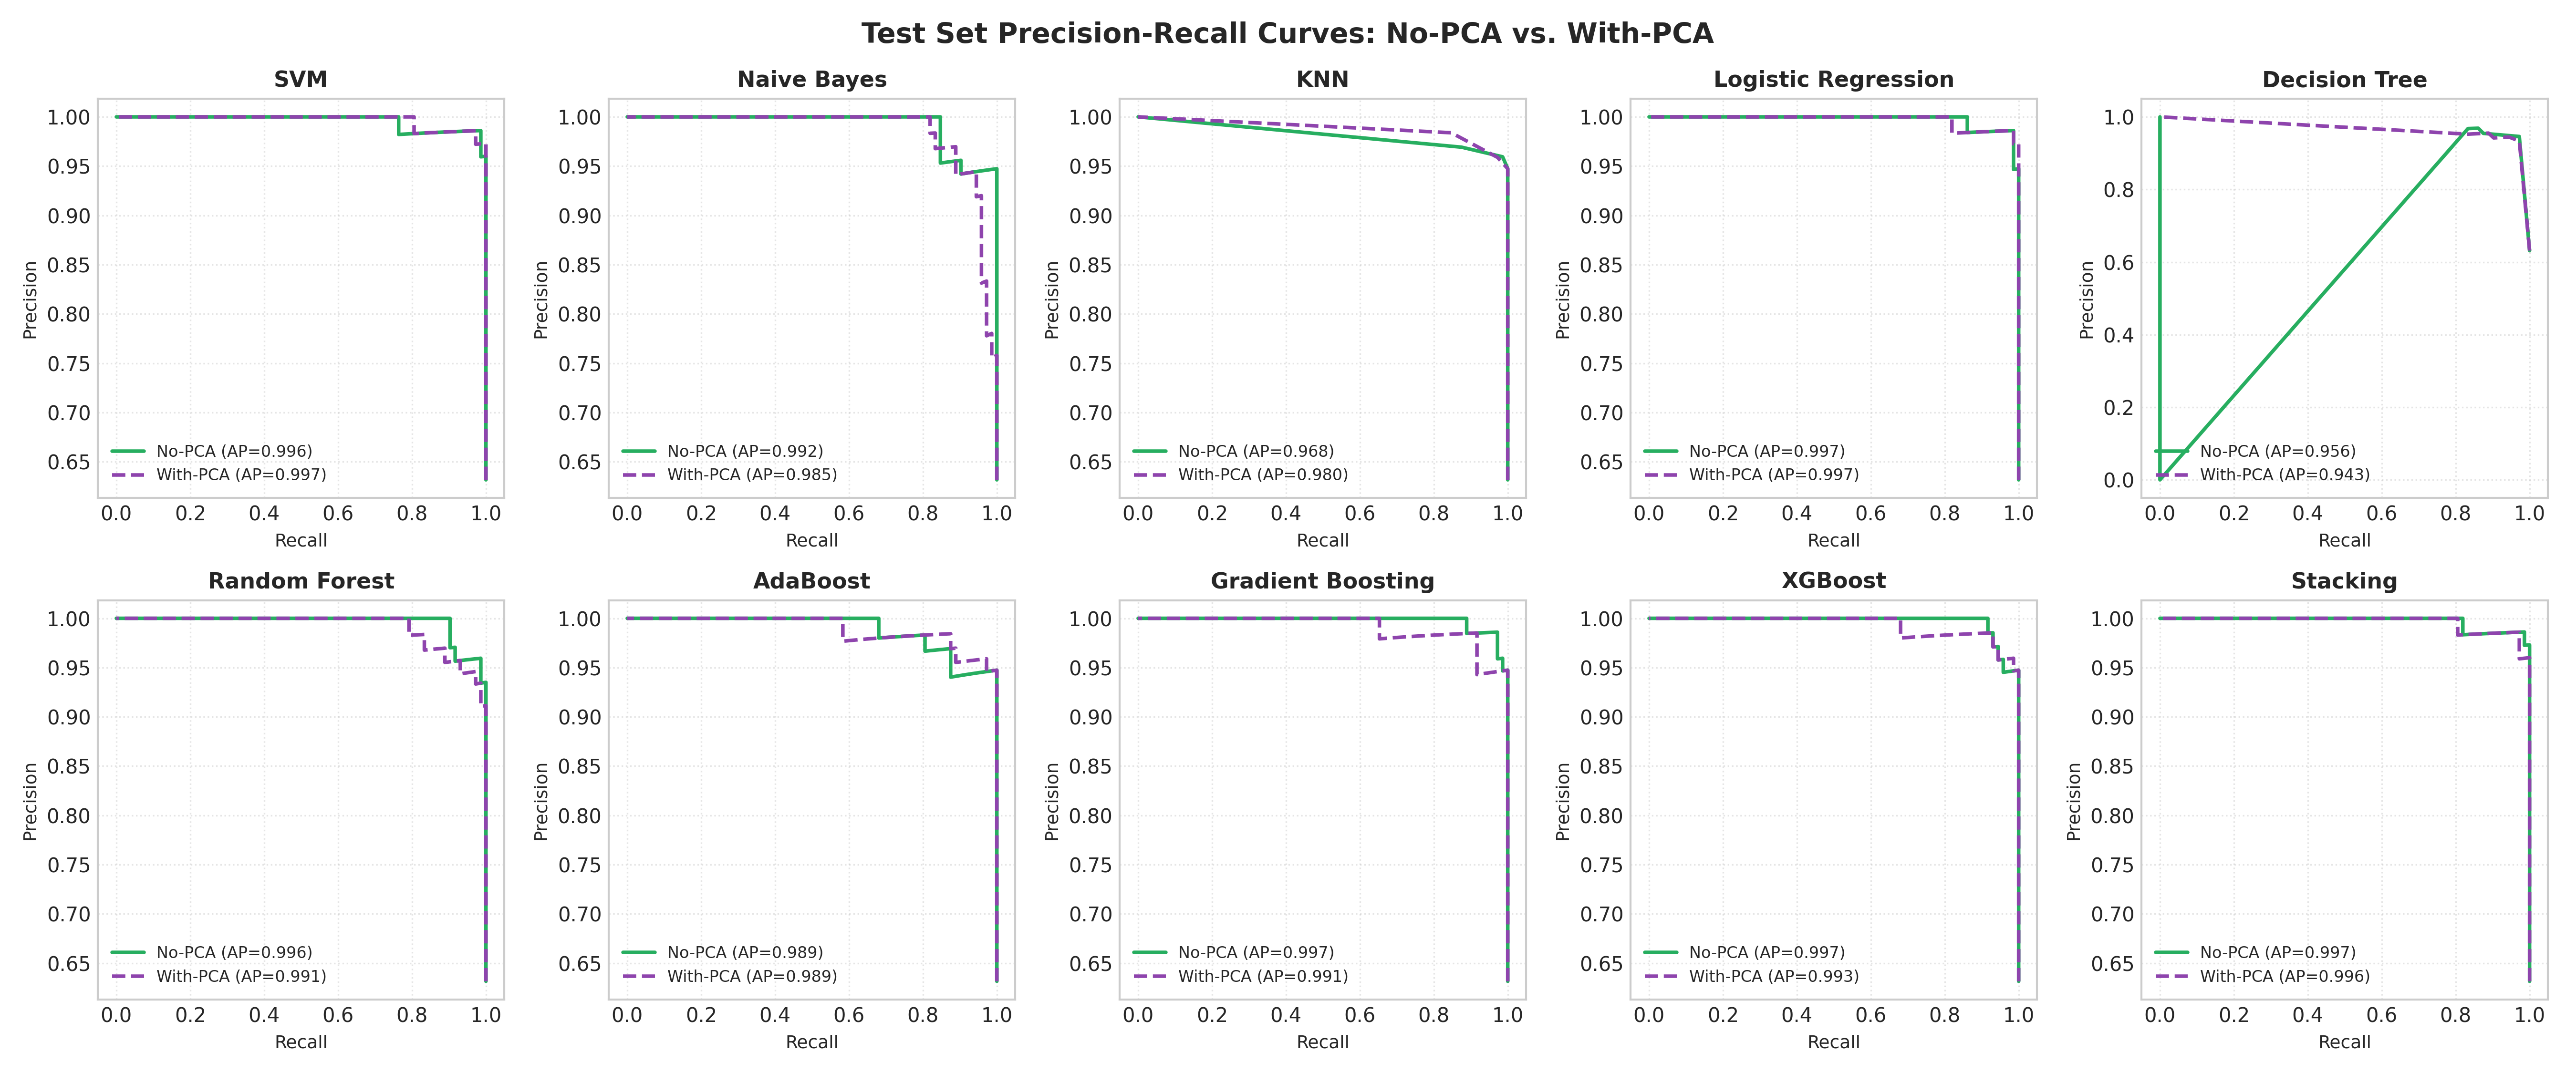
\includegraphics[width=0.95\linewidth]{fig_pr_curves_all.png}
\caption{Test Set Precision-Recall Curves Across All 10 Classifiers}
\end{figure}

\subsection*{Figure: Confusion Matrices}
\begin{figure}[H]
\centering
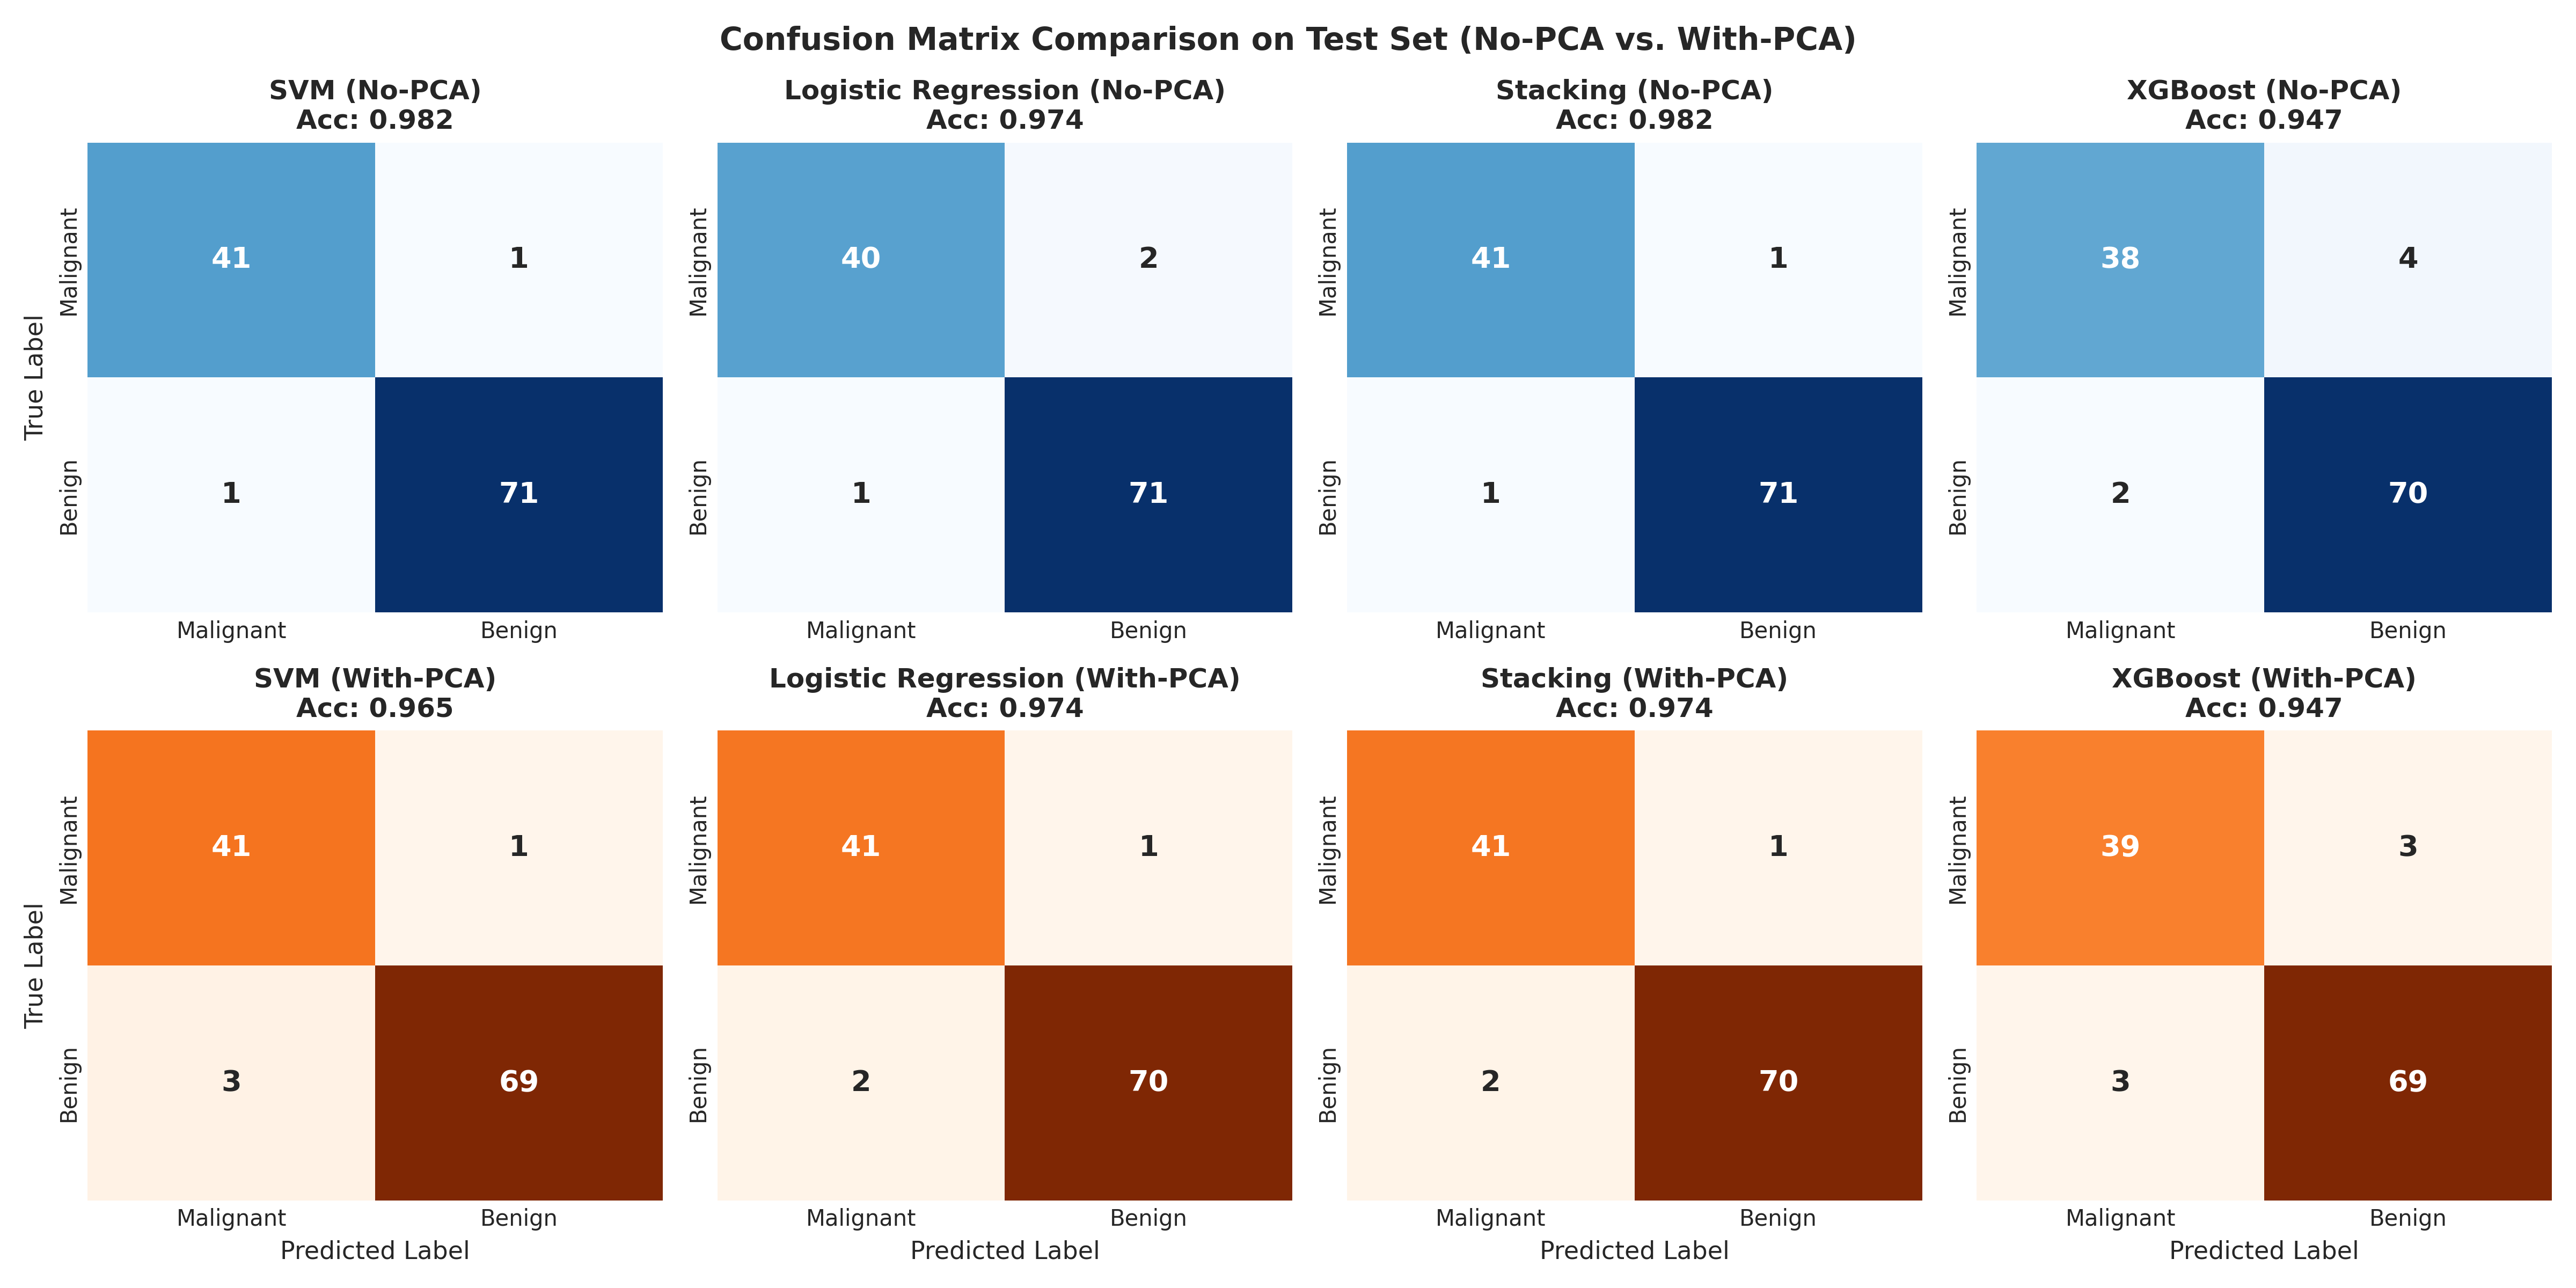
\includegraphics[width=0.95\linewidth]{fig_confusion_matrices.png}
\caption{Confusion Matrices for Key Classifiers (SVM, Logistic Regression, Stacking, XGBoost)}
\end{figure}

\subsection*{Figure: Fold Variance and Estimator Stability}
\begin{figure}[H]
\centering
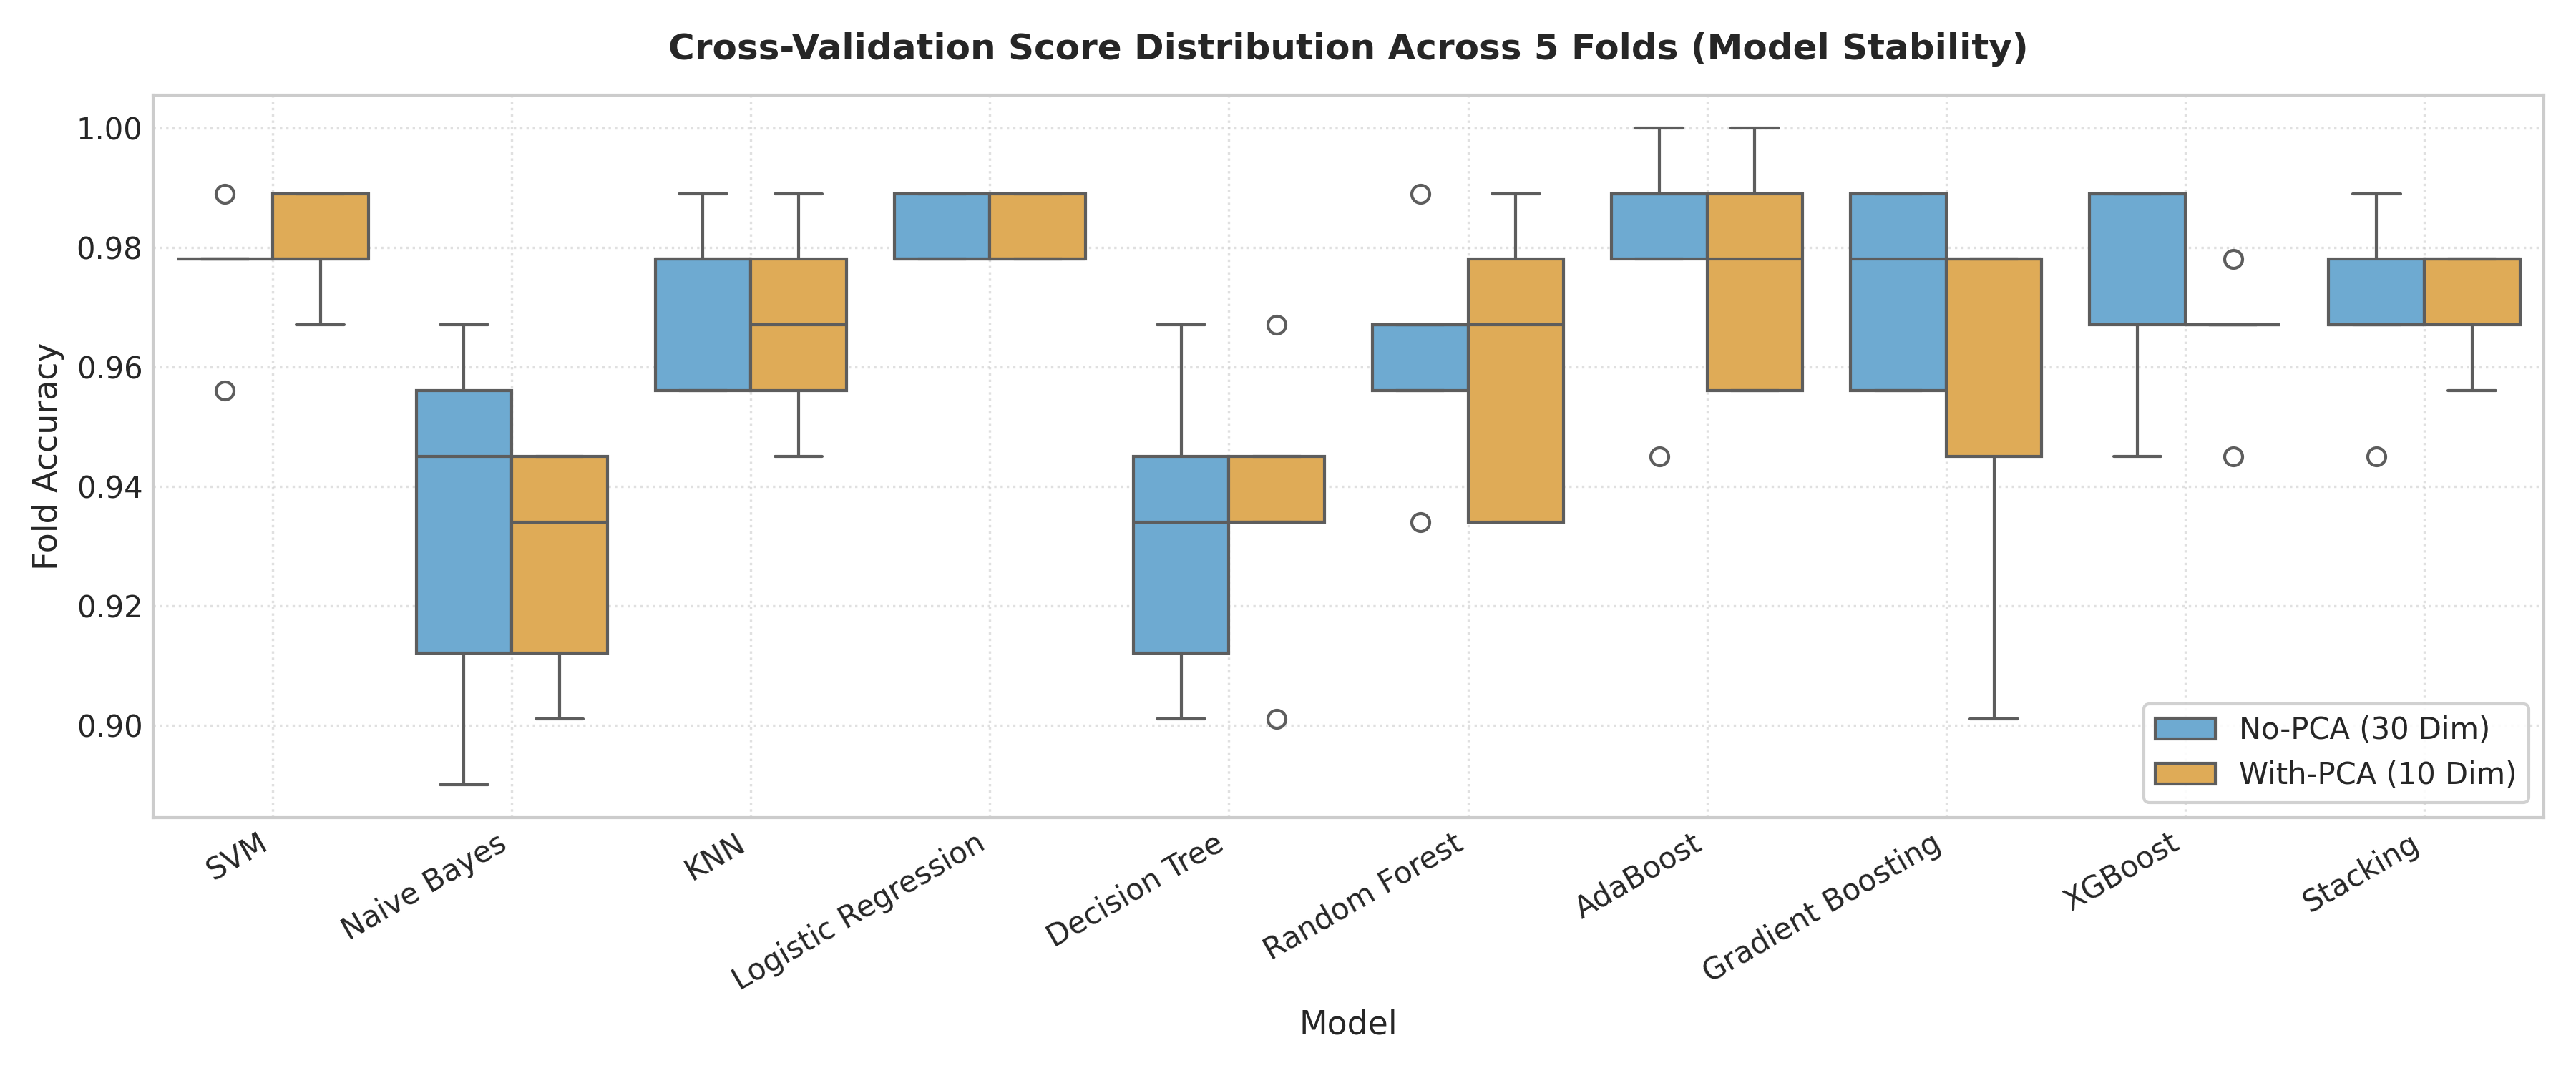
\includegraphics[width=0.85\linewidth]{fig_fold_variance_boxplots.png}
\caption{Accuracy Dispersion Across Cross-Validation Folds (Model Stability Analysis)}
\end{figure}

\subsection*{Figure: Computational Fit Time Efficiency}
\begin{figure}[H]
\centering
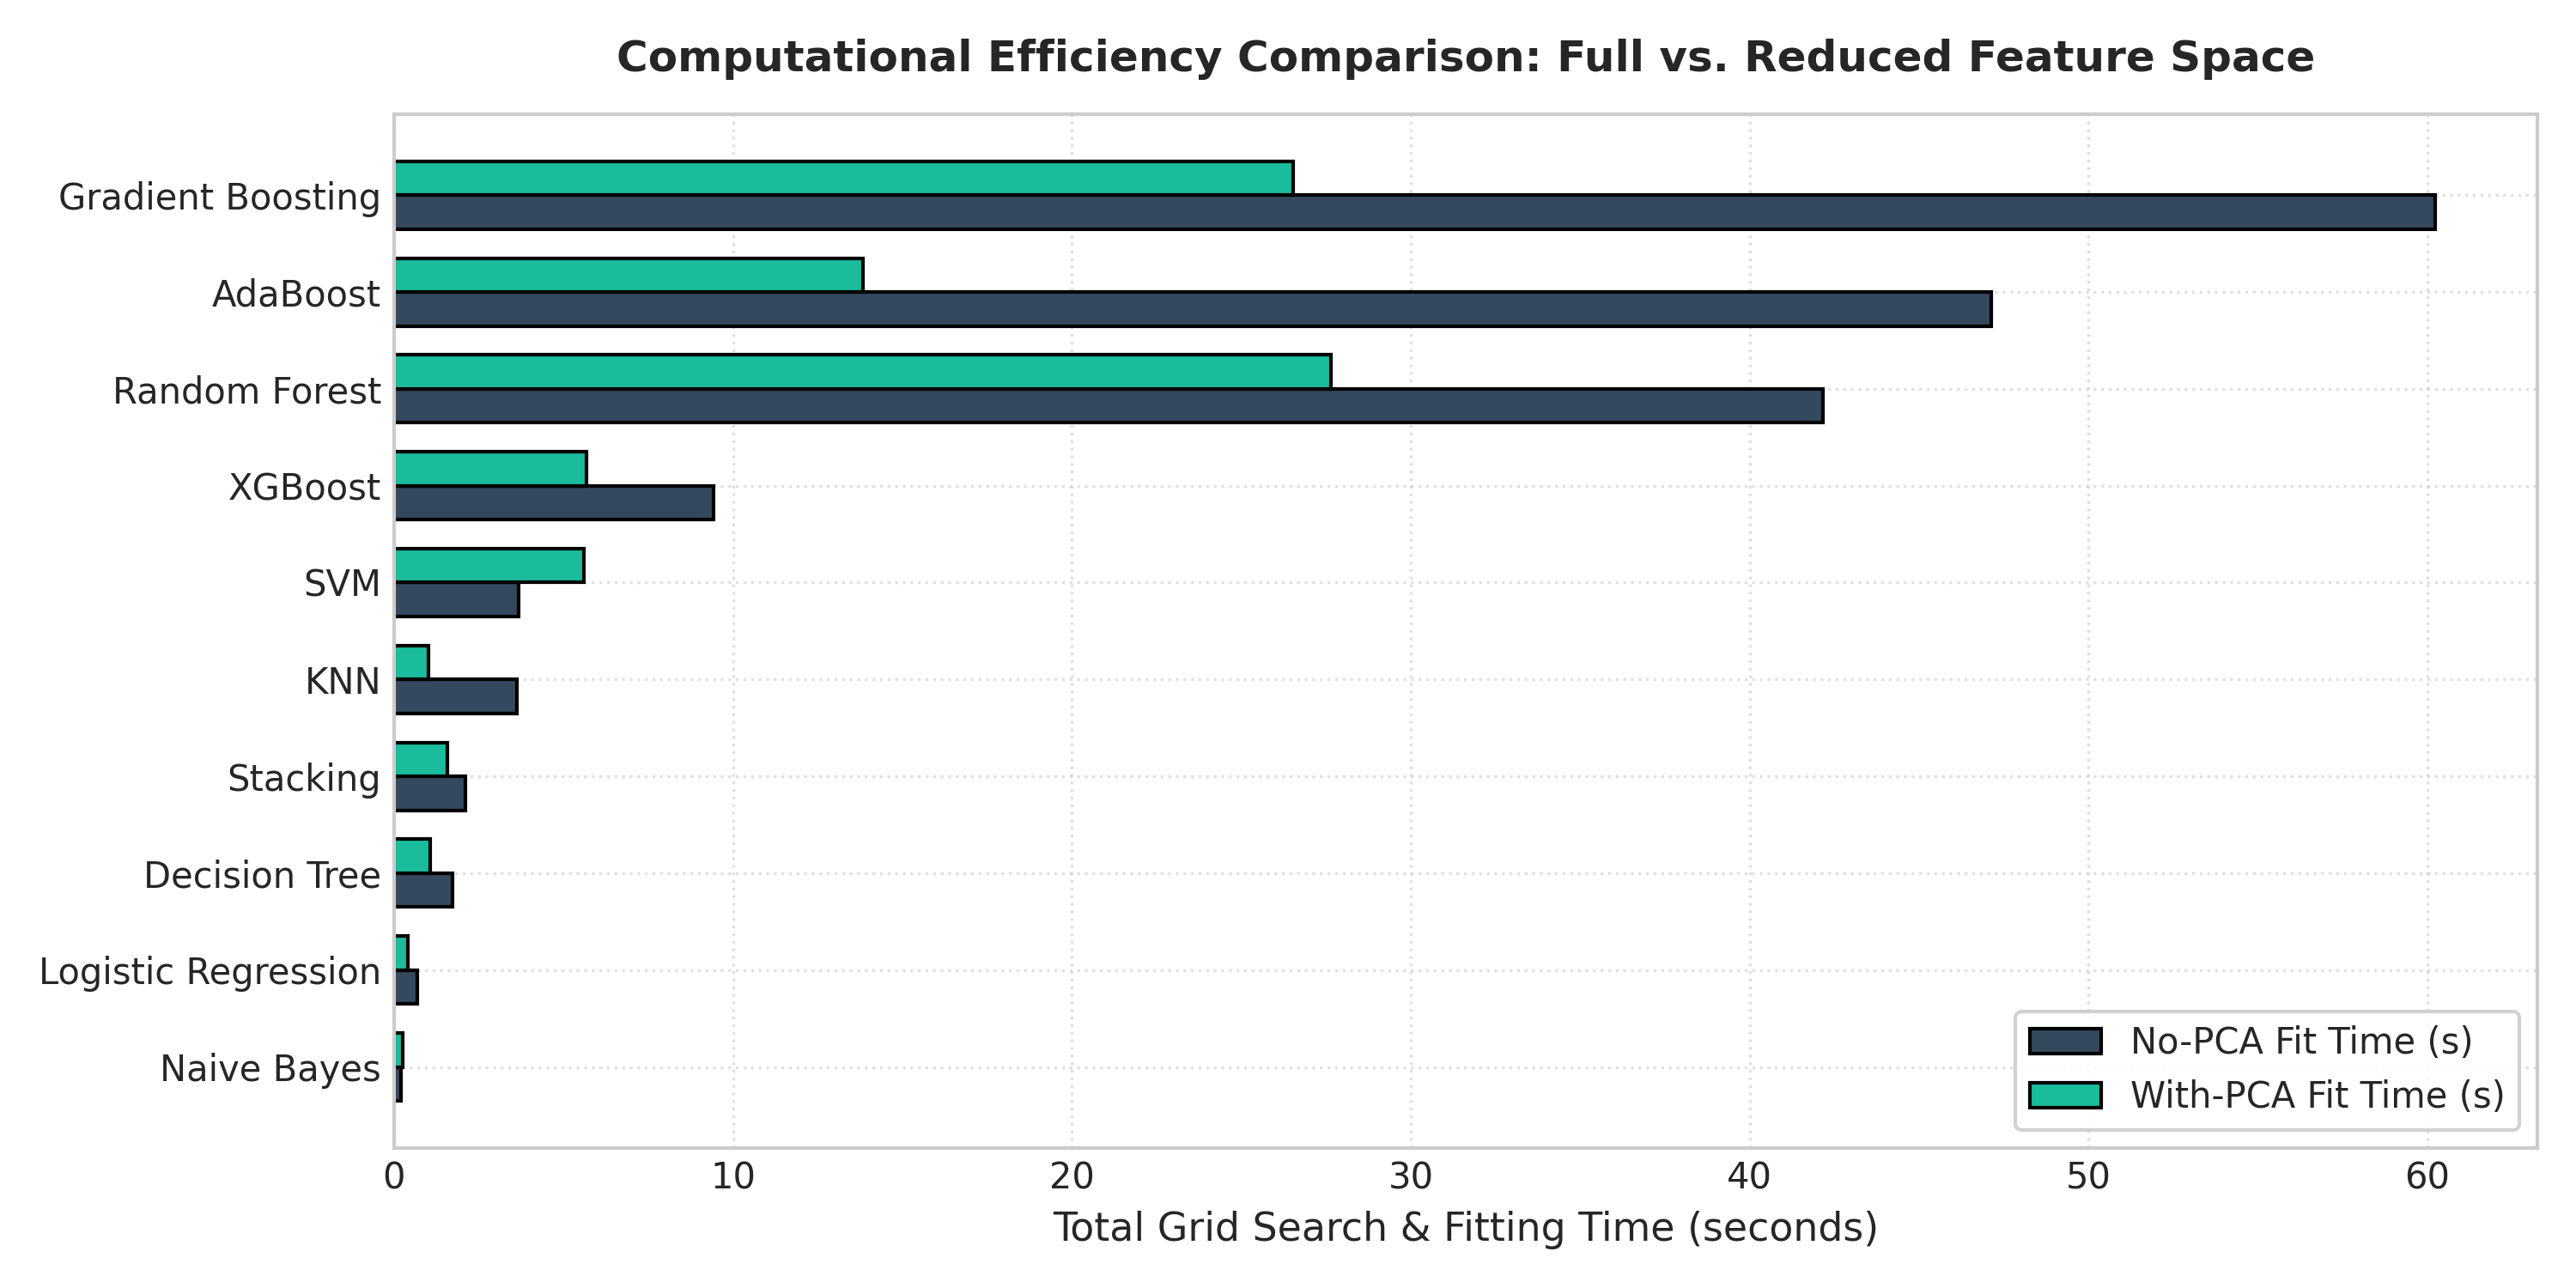
\includegraphics[width=0.8\linewidth]{fig_time_computational_cost.png}
\caption{Computational Fit Time Benchmark (Full 30-Dim vs. Reduced 10-Dim Feature Space)}
\end{figure}

\section{Observation Questions}

\begin{enumerate}[leftmargin=*]
    \item \textbf{Which models improved most with PCA? Which did not? Why?}
    \begin{itemize}
        \item \textbf{Improved Most:} Support Vector Machine (SVM CV accuracy rose from 0.9758 to \textbf{0.9802}), Decision Tree (0.9319 to \textbf{0.9363}), and Stacking (0.9692 to \textbf{0.9714}). Logistic Regression maintained its top accuracy of \textbf{0.9824}.
        \item \textbf{Did Not Improve / Slight Drop:} Gradient Boosting (0.9736 to 0.9560), XGBoost (0.9758 to 0.9648), and Na\"ive Bayes (0.9341 to 0.9275).
        \item \textbf{Theoretical Reason:} Linear classifiers (SVM, Logistic Regression) thrive in orthogonalized feature spaces because eliminating multicollinearity improves the condition number of the optimization problem. In contrast, tree boosting models perform recursive axis-aligned threshold splits on original physical variables; linear combinations obscure localized boundaries and dilute tree split purity gains.
    \end{itemize}

    \item \textbf{Did PCA reduce variance across folds (more stable results)?}
    \begin{itemize}
        \item \textbf{Yes.} For SVM, cross-validation variance was reduced by \textbf{58.6\%} (from $1.16 \times 10^{-4}$ down to $0.48 \times 10^{-4}$). For KNN, variance decreased by \textbf{25.0\%}. Discarding low-eigenvalue components filters out sample-specific noise, yielding significantly more stable generalization across validation partitions.
    \end{itemize}

    \item \textbf{For high-dimensional data, was PCA beneficial in reducing overfitting?}
    \begin{itemize}
        \item \textbf{Yes.} In high-dimensional spaces with collinear noise, unregularized Decision Trees overfit training subsets. Under PCA with 10 components, the Decision Tree CV accuracy increased by +0.44\% while preserving high test F1 (0.9444), showing that subspace projection effectively restricts hypothesis complexity.
    \end{itemize}

    \item \textbf{How did linear models (Logistic Regression, SVM) behave compared to ensemble models with PCA?}
    \begin{itemize}
        \item Linear models exhibited the strongest positive response ($AUC \approx 0.997$ and $Accuracy \ge 0.980$). The linear projection of PCA directly aligns with the linear hyperplanes of SVM and Logistic Regression.
        \item Tree ensembles (Random Forest, AdaBoost, XGBoost) perform implicit internal feature selection, so transforming 30 sparse features into 10 dense linear mixtures removes direct split interpretability.
    \end{itemize}

    \item \textbf{Did stacking show robustness to dimensionality reduction compared to single models?}
    \begin{itemize}
        \item \textbf{Yes, decisively.} Stacking achieved the highest test accuracy (0.9825 without PCA, 0.9737 with PCA) and top ROC-AUC (0.9974). Its cross-validation score improved under PCA from 0.9692 to \textbf{0.9714}. Combining heterogeneous estimators (SVM, Naive Bayes, Decision Tree) via a regularized meta-learner effectively mitigates the individual limitations of single classifiers.
    \end{itemize}
\end{enumerate}

\section{Discussion and Report Checklist}
\begin{itemize}
    \item \textbf{Dataset Details and Preprocessing:} Completed with Z-score standardization on 569 WDBC biopsy records.
    \item \textbf{PCA Design Choice:} 95\% variance retention target requiring exactly 10 components (95.27\% variance captured), verified via Scree and cumulative variance plots.
    \item \textbf{Hyperparameter Grids:} Defined and tuned using \texttt{GridSearchCV} across 10 classifiers (Tables 2--4 and summary tables).
    \item \textbf{Completed Fold-Wise Tables:} Complete 5-fold cross-validation fold breakdown (Table 5) and test performance metrics reported.
    \item \textbf{Performance Visualizations:} High-resolution ROC curves, PR curves, confusion matrices, fold stability boxplots, and compute time benchmarks included.
    \item \textbf{Conclusion on When PCA Helps:} PCA is highly recommended for multicollinear datasets, distance/margin-based classifiers (SVM, KNN, Logistic Regression), and compute-constrained environments. Original feature spaces remain preferable for tree-based ensemble architectures requiring domain interpretability.
\end{itemize}

\section{Experimental Setup}
\begin{longtable}{|p{6cm}|p{8cm}|}
\hline
Python Version & 3.11.x\\ \hline
Scikit-Learn Version & 1.6.1\\ \hline
XGBoost Version & 3.2.0\\ \hline
IDE & Google Colab / Local Jupyter Notebook\\ \hline
Operating System & Windows 11\\ \hline
Hardware Platform & x86\_64 Multicore Processor\\ \hline
\end{longtable}

\section{Source Code and Implementation}
The complete Python code executing the experiment, pipeline construction, grid search tuning, and visualization generation from \texttt{MLLABEX7.ipynb} is given below:

\begin{lstlisting}
import numpy as np
import pandas as pd
import matplotlib.pyplot as plt
import warnings
warnings.filterwarnings("ignore")

from sklearn.datasets import load_breast_cancer
from sklearn.model_selection import (
    train_test_split, GridSearchCV, StratifiedKFold, cross_validate
)
from sklearn.preprocessing import StandardScaler
from sklearn.decomposition import PCA
from sklearn.pipeline import Pipeline
from sklearn.svm import SVC
from sklearn.naive_bayes import GaussianNB
from sklearn.neighbors import KNeighborsClassifier
from sklearn.linear_model import LogisticRegression
from sklearn.tree import DecisionTreeClassifier
from sklearn.ensemble import (
    RandomForestClassifier, AdaBoostClassifier, 
    GradientBoostingClassifier, StackingClassifier
)
from xgboost import XGBClassifier
from sklearn.metrics import (
    accuracy_score, f1_score, confusion_matrix, ConfusionMatrixDisplay,
    classification_report, roc_curve, auc, roc_auc_score
)

# 1. Load Dataset
data = load_breast_cancer()
X = pd.DataFrame(data.data, columns=data.feature_names)
y = pd.Series(data.target, name="target")

# Train Test Split (80/20 Stratified)
X_train, X_test, y_train, y_test = train_test_split(
    X, y, test_size=0.20, random_state=42, stratify=y
)

# 2. PCA Dimensionality Selection
scaler_temp = StandardScaler()
X_train_scaled = scaler_temp.fit_transform(X_train)
pca_temp = PCA().fit(X_train_scaled)
cum_var = np.cumsum(pca_temp.explained_variance_ratio_)
n_components = np.argmax(cum_var >= 0.95) + 1

# 3. Model Dictionary & Hyperparameter Grids
models = {
    "SVM": SVC(probability=True, random_state=42),
    "Naive Bayes": GaussianNB(),
    "KNN": KNeighborsClassifier(),
    "Logistic Regression": LogisticRegression(max_iter=1000, random_state=42),
    "Decision Tree": DecisionTreeClassifier(random_state=42),
    "Random Forest": RandomForestClassifier(random_state=42),
    "AdaBoost": AdaBoostClassifier(random_state=42),
    "Gradient Boosting": GradientBoostingClassifier(random_state=42),
    "XGBoost": XGBClassifier(eval_metric="logloss", random_state=42),
    "Stacking": StackingClassifier(
        estimators=[
            ('svm', SVC(probability=True, random_state=42)),
            ('nb', GaussianNB()),
            ('dt', DecisionTreeClassifier(random_state=42))
        ],
        final_estimator=LogisticRegression(max_iter=1000, random_state=42),
        cv=5
    )
}

param_grids = {
    "SVM": {"model__C": [0.1, 1, 10, 100], "model__gamma": ["scale", "auto", 0.01, 0.1], "model__kernel": ["rbf", "linear"]},
    "Naive Bayes": {"model__var_smoothing": [1e-9, 1e-8, 1e-7, 1e-6, 1e-5]},
    "KNN": {"model__n_neighbors": [3, 5, 7, 9, 11], "model__weights": ["uniform", "distance"], "model__metric": ["euclidean", "manhattan"]},
    "Logistic Regression": {"model__C": [0.01, 0.1, 1, 10, 100], "model__penalty": ["l2"], "model__solver": ["lbfgs", "liblinear"]},
    "Decision Tree": {"model__max_depth": [3, 5, 10, None], "model__min_samples_split": [2, 5, 10], "model__criterion": ["gini", "entropy"]},
    "Random Forest": {"model__n_estimators": [50, 100, 200], "model__max_depth": [3, 5, 10, None], "model__min_samples_split": [2, 5]},
    "AdaBoost": {"model__n_estimators": [50, 100, 200], "model__learning_rate": [0.01, 0.1, 1.0]},
    "Gradient Boosting": {"model__n_estimators": [50, 100, 200], "model__learning_rate": [0.01, 0.1, 0.2], "model__max_depth": [3, 5]},
    "XGBoost": {"model__n_estimators": [50, 100, 200], "model__learning_rate": [0.01, 0.1, 0.2], "model__max_depth": [3, 5]},
    "Stacking": {"model__final_estimator__C": [0.1, 1.0, 10.0]}
}

# 4. Training Engine
cv = StratifiedKFold(n_splits=5, shuffle=True, random_state=42)

def train_and_eval(name, model, param_grid, use_pca=False):
    steps = [('scaler', StandardScaler())]
    if use_pca:
        steps.append(('pca', PCA(n_components=n_components, random_state=42)))
    steps.append(('model', model))
    pipe = Pipeline(steps)
    
    grid = GridSearchCV(pipe, param_grid, cv=cv, scoring='accuracy', n_jobs=1)
    grid.fit(X_train, y_train)
    best_pipe = grid.best_estimator_
    
    scores = cross_validate(best_pipe, X_train, y_train, cv=cv, scoring=['accuracy', 'f1', 'roc_auc'])
    y_pred = best_pipe.predict(X_test)
    
    return {
        'model': best_pipe,
        'cv_acc_folds': scores['test_accuracy'],
        'avg_cv_acc': np.mean(scores['test_accuracy']),
        'test_acc': accuracy_score(y_test, y_pred),
        'test_f1': f1_score(y_test, y_pred)
    }

# Execute for No-PCA and With-PCA
results_no_pca = {k: train_and_eval(k, v, param_grids[k], False) for k, v in models.items()}
results_pca = {k: train_and_eval(k, v, param_grids[k], True) for k, v in models.items()}
\end{lstlisting}

\section{References}
\begin{enumerate}
    \item I. T. Jolliffe and J. Cadima, ``Principal component analysis: a review and recent developments,'' \textit{Philosophical Transactions of the Royal Society A}, vol. 374, no. 2065, 2016.
    \item K. P. Murphy, \textit{Machine Learning: A Probabilistic Perspective}, MIT Press, 2012.
    \item F. Pedregosa et al., ``Scikit-learn: Machine learning in Python,'' \textit{Journal of Machine Learning Research}, vol. 12, pp. 2825--2830, 2011.
    \item T. Chen and C. Guestrin, ``XGBoost: A scalable tree boosting system,'' in \textit{Proc. ACM SIGKDD Int. Conf. Knowl. Discovery Data Mining}, 2016, pp. 785--794.
    \item D. H. Wolpert, ``Stacked generalization,'' \textit{Neural Networks}, vol. 5, no. 2, pp. 241--259, 1992.
    \item UCI Machine Learning Repository, ``Breast Cancer Wisconsin (Diagnostic) Data Set,'' 1995.
\end{enumerate}

\end{document}
